\documentclass[10pt,mathserif,aspectratio=169]{beamer}
\usepackage{graphicx,amsmath,verbatim}   % amssymb omitted: newtxmath supplies the AMS symbols,
                                          % and loading both exhausts the 16 math alphabets
\usepackage{mathtools}      % \mathclap for wide underbrace labels
\usepackage{tikz}
\usepackage{pgfplots}
\usepackage{array}
\usepackage{hyperref}
\usepackage{booktabs}
\usepackage[normalem]{ulem}
\usepackage{longtable}
\usepackage{subcaption}
\usepackage{blkarray}
\usepackage{nicematrix}     % cell shading for the permuted-dense figures
\usepackage{appendixnumberbeamer}
\graphicspath{{./images/}{./plans/}}
\usepackage{adjustbox}   % max size={..}{..}: shrink a figure to fit, never enlarge it
\usetikzlibrary{shapes.geometric}
\usetikzlibrary{arrows}
\pgfplotsset{compat=1.17}
\usepgfplotslibrary{groupplots}
\usetikzlibrary{calc,patterns,decorations.pathmorphing,decorations.markings,arrows.meta}
\usetikzlibrary{positioning,fit,backgrounds}
\usetikzlibrary{overlay-beamer-styles} % provides the `alt=<n>{..}{..}` overlay key

% NOTE: \tikzexternalize is deliberately NOT used. The figures/ directory does not exist,
% and the overlay frames have to re-render on every slide anyway.

% ---------------------------------------------------------------------------------------
% Math alphabet budget. A math version may use at most 16 alphabets under pdfTeX.
% newtxmath claims 6 and bm claims 4, which leaves nothing for the thesis notation
% (\mmat = \mathbf, \cone = \mathcal, \reals = \mathbb, plus \mathrm) in one formula.
% bm is only needed for \gvec, so we pre-empt it and route \gvec through amsmath's
% \boldsymbol, which costs no alphabet in the normal version. Leaves 14 of 16 in use.
\usepackage{amsbsy}
\makeatletter \@namedef{ver@bm.sty}{2019/07/24} \makeatother
\providecommand{\bm}[1]{\boldsymbol{#1}}
% ---------------------------------------------------------------------------------------

\input defs.tex
\input listing_defs.tex
\lstset{numbers=none}       % line numbers are noise on a slide

\bibliographystyle{apalike}

% comment out the following three lines to get default beamer fonts
\usepackage{newtxtext}
\usepackage{newtxmath}
\renewcommand{\familydefault}{\sfdefault}


%% formatting

\mode<presentation>
{
\usetheme{default}
}
\setbeamertemplate{navigation symbols}{}
% Slide number, bottom right, quiet enough to ignore while presenting and readable from the
% floor when someone asks "could you go back to the one with the table?". appendixnumberbeamer
% (loaded above) keeps the backups out of it: in the main deck the denominator is the number
% of slides that will actually be presented, and the appendix restarts its own count, so the
% total never advertises ten backup slides the talk does not reach. The title page carries no
% number -- it is \frame[plain], which drops the footline.
\setbeamertemplate{footline}{%
  \hfill{\scriptsize\color{black!40}%
  \insertframenumber\,/\,\inserttotalframenumber}\hspace{2.5ex}\vspace{1.5ex}}
\usecolortheme[rgb={0.13,0.28,0.59}]{structure}
\setbeamertemplate{itemize subitem}{--}
\setbeamertemplate{frametitle} {
  \vspace*{2ex}
  {\large\bfseries \insertframetitle}
}

% one breath between top-level bullets, everywhere
\newcommand{\bul}{\setlength\itemsep{1.1ex}}

% One outline frame at the start of every section, as a break between them: five in all,
% with the section being entered highlighted and the rest greyed. Restored 2026-09-16 after
% a spell with a single outline frame after the title page -- that one is gone, since it
% would have rendered immediately before this one fires for Introduction and the two read
% as the same slide twice. The cost is four extra slides against the single-outline version;
% at a 30-minute slot that is the trade being made knowingly.
\AtBeginSection[]{%
  \begin{frame}{Outline}
  \vfill
  \tableofcontents[currentsection,currentsubsection]
  \vfill
  \end{frame}}

% colours of the permuted-dense figures, matching the thesis
\colorlet{pdBlock}{blue!22}
\colorlet{pdRowA}{blue!22}
\colorlet{pdRowB}{green!28!white}
\colorlet{pdRowC}{orange!38!white}
\colorlet{pdRowD}{purple!26!white}

% Square brackets around a 3x3 grid of 0.62cm cells whose top-left centre is at (#1, 0).
% Defined here, not inside the frame: a #1 inside the \fitfig{} argument is misparsed.
\newcommand{\pdbrackets}[1]{%
  \draw[brk] (#1-0.36, 0.34) -- (#1-0.47, 0.34) -- (#1-0.47, -1.58) -- (#1-0.36, -1.58);
  \draw[brk] (#1+1.60, 0.34) -- (#1+1.71, 0.34) -- (#1+1.71, -1.58) -- (#1+1.60, -1.58);}

% Fit a big figure to the frame: shrinks when needed, never enlarges.
\newcommand{\fitfig}[1]{\adjustbox{max size={0.98\textwidth}{0.70\textheight}}{#1}}

% --- the level-2 strip, recalled on the worked-example slides -------------------------
% Same four words, order and spacing as the strips of I1/F0/I1b, so the example slides say
% where in the pipeline each beat sits. #1 selects the current box:
%   1 convex problem   2 compilation   3 conic form   4 solver
\newcommand{\stripsel}[2]{\ifnum#1=#2 hlbox\else dimbox\fi}
% #1 (optional) renames the first box, for a slide where the artifact on screen has a
% more specific name than `convex problem'. The bar is set to a fixed width, so the
% substitute word does not change its size.
\newcommand{\recallstrip}[2][convex problem]{%
  \vspace{-2ex}%
  \begin{center}%
  \adjustbox{width=0.60\textwidth}{%
  \begin{tikzpicture}
    \node[\stripsel{#2}{1}] (r1) at (0,0)   {#1};
    \node[\stripsel{#2}{2}] (r2) at (2.4,0) {compilation};
    \node[\stripsel{#2}{3}] (r3) at (4.8,0) {conic form};
    \node[\stripsel{#2}{4}] (r4) at (7.2,0) {solver};
    \draw[dimflow] (r1) -- (r2);  \draw[dimflow] (r2) -- (r3);
    \draw[dimflow] (r3) -- (r4);
  \end{tikzpicture}}%
  \end{center}%
  \vspace{0.5ex}}

% --- pipeline-diagram visual grammar (intro slides) ------------------------------------
% Two node roles, used at all three zoom levels:
%   art   an artifact: a thing that exists  (the problem, the conic form, P/A/b/c)
%   proc  a process: a thing that acts      (modelling, solver)
% Transformations are labelled arrows (flow + edgelab), so each zoom level can reveal a
% new `art` box inside what the previous level drew as a single arrow.
\definecolor{polyblue}{rgb}{0.13,0.28,0.59}   % the beamer structure colour
\tikzset{
  art/.style     ={draw=black!55, fill=polyblue!7,  inner sep=6pt, font=\small},
  proc/.style    ={draw=black!55, fill=polyblue!22, rounded corners=3pt,
                   minimum height=8mm, inner xsep=6pt, font=\small},
  flow/.style    ={-{Stealth[length=2.2mm]}, thick, draw=black!70},
  edgelab/.style ={font=\footnotesize, midway, above=0.5mm},
  ends/.style    ={font=\small\itshape, text=black!55, align=center},
  note/.style    ={font=\footnotesize, text=black!55, align=center},
  % the greyed carry-over strip at the top of the two zoom slides
  dimbox/.style  ={draw=black!25, fill=black!3, rounded corners=2pt,
                   inner sep=3pt, font=\scriptsize, text=black!50},
  dimflow/.style ={-{Stealth[length=1.6mm]}, draw=black!30},
  zoombox/.style ={draw=polyblue, dashed, thick, rounded corners=2pt, inner sep=3pt},
  zoomline/.style={draw=polyblue!60, dashed},
  accent/.style  ={draw=polyblue, very thick},   % the one arrow that is "this thesis"
  % an annotation box hanging off a pipeline box: dashed, so it does not read as a stage
  exbox/.style   ={draw=black!40, dashed, fill=white, rounded corners=2pt,
                   inner sep=5pt, font=\footnotesize, align=left},
  % a standing box that fills space rather than annotating one node: solid, titled,
  % and tinted in the same blue family as the pipeline boxes it unpacks -- art!7 for
  % what the solver does, proc!22 for who implements it, so the `solvers' box carries
  % the colour of the solver node itself
  bigbox/.style  ={draw=polyblue!55, fill=polyblue!7, rounded corners=3pt,
                   inner sep=7pt, minimum height=15mm, font=\footnotesize,
                   align=left, text width=5.9cm},
  boxtitle/.style={font=\footnotesize\bfseries, text=polyblue},
  % the current box of the recall strip on the worked-example slides
  hlbox/.style   ={draw=polyblue, fill=polyblue!12, rounded corners=2pt,
                   inner sep=3pt, font=\scriptsize, text=polyblue},
  % --- sparsity-pattern figure (I4) ---------------------------------------------
  % The picture is drawn in cell units (x=y=0.09cm on the tikzpicture), so dot radii
  % are given in absolute units and survive the \fitfig rescale.
  nz/.style       ={fill=polyblue, draw=none},        % one nonzero
  matframe/.style ={draw=black!60, thin},             % the outline of the matrix
}


% shorthands used throughout the deck
\newcommand{\sde}{\texttt{SparseDiffEngine}}
\newcommand{\sdp}{\texttt{sparsediffpy}}
\newcommand{\de}{\texttt{diffengine}}
\newcommand{\cvxpy}{\texttt{CVXPY}}

\title{\large \bfseries A Lightweight Canonicalization Engine in C\\
for Disciplined Convex Programming}

\author{William Zijie Zhang}

\date{Master's Thesis Defence \\[0.5ex]
      {October 2nd}}

\begin{document}

% =====================================================================================
%  Slides start here.
%
%  Preamble conventions, so they do not have to be rediscovered:
%    \fitfig{<tikzpicture>}   shrink a figure to fit the frame; never enlarges
%    \bul                     first thing inside an itemize: one breath between bullets
%    \cvxpy{}                 CVXPY          \sde{}  SparseDiffEngine
%    \sdp{}                   sparsediffpy   \de{}   diffengine
%    \mvec{x} \mmat{A} \gvec{\theta} \cone{K} \reals \zeros    thesis notation (defs.tex)
%    \annotatedop{op}{expr}   tree node with a grey annotation to its right
%    pdBlock, pdRowA..pdRowD  the permuted-dense figure colours
%    nz, matframe             the sparsity-pattern figure (I4)
%
%    \begin{frame}[fragile]   REQUIRED on any frame containing a lstlisting
%    visible on=<2->          on a tikz scope: stage a reveal without moving the figure
%    \item<2->  \item<2->[--] reveal a bullet, marker and all, with its space reserved
%                             (I0b, F2). \onslide inside an \item leaves the marker behind.
%    \only<1>{..}\only<2>{..} two versions of one block, e.g. B3's two beats. Keep the two
%                             metrically identical or \fitfig rescales between the beats.
%
%  One Outline frame opens every section -- five in all, fired by \AtBeginSection (line 84),
%  which the \section commands only trigger. I0 sits before the first of them, between the
%  title page and \section{Introduction}: see its own comment for why.
% =====================================================================================

\frame[plain]{
\thispagestyle{empty}
\titlepage
\vspace{-4ex}
\begin{center}\footnotesize
Research director: Antoine Lesage-Landry \\[0.5ex]
Department of Electrical Engineering, Polytechnique Montr\'eal
\end{center}
}

% --- I0 -------------------------------------------------------------------------
%  Zoom level 1: how optimization gets done at all. Deliberately before the first Outline
%  frame rather than after it: the deck opens on the picture the whole talk lives inside,
%  and the outline then reads as a route through a landscape the room has already been
%  shown. It is the only frame outside a section, which costs nothing -- \AtBeginSection
%  (line 84) fires on \section{Introduction} just below, so the Outline still lands second.
%
%  Two beats, following the same grammar as I1b below: the chain names its stages, then a
%  dashed annotation box hangs off one of them to say what that stage actually contains.
%  To stage a left-to-right build instead, add `visible on=<2->' to individual nodes.
%
%  `modelling language' hangs off the formulation -> solver arrow as an exbox, and is not a
%  sixth box of the chain. It was drawn as a `proc' stage first and that was wrong twice
%  over: it widened the chain to 16.4 units, which \fitfig pays for by shrinking every label
%  on the slide, and it put the thing the whole deck is about on the same footing as
%  `modelling' and `solver', which this slide is not yet ready to justify. As an annotation
%  it says the more useful thing -- the arrow is where it lives -- and it leaves the level-1
%  chain at five boxes, which is what I1's carry-over strip repeats.
%
%  Bullet 1 is the declarative framing, said the way Boyd says it: the model states what you
%  want, not how to get it. It is what the thesis opens on too, in the historical register --
%  modellers think in sets, indices and algebraic expressions while procedural code builds
%  the coefficient matrices entry by entry (5-Introduction.tex:11-14).
%  Bullet 2 is <2->, so it lands with the exbox rather than ahead of it. It names what the
%  new box is for and is the sentence the rest of the deck is about. `bridge' is meant in
%  its plain sense; MOI's technical `bridge' (6-Revue_litterature.tex:1037-1040) is a
%  different object that the deck never draws, though MOI is named on I1b.
%  Two lines were considered and are not written. "everything after it is mechanical" --
%  the chain draws it, and bullet 2 says the useful half. "this talk is not about how to
%  model problems, nor how to solve them, but everything in between" -- right content, wrong
%  register: no other frame in the deck talks about the talk. Both are worth saying aloud.
\begin{frame}{Optimization in practice}
\vfill
\begin{center}
\fitfig{%
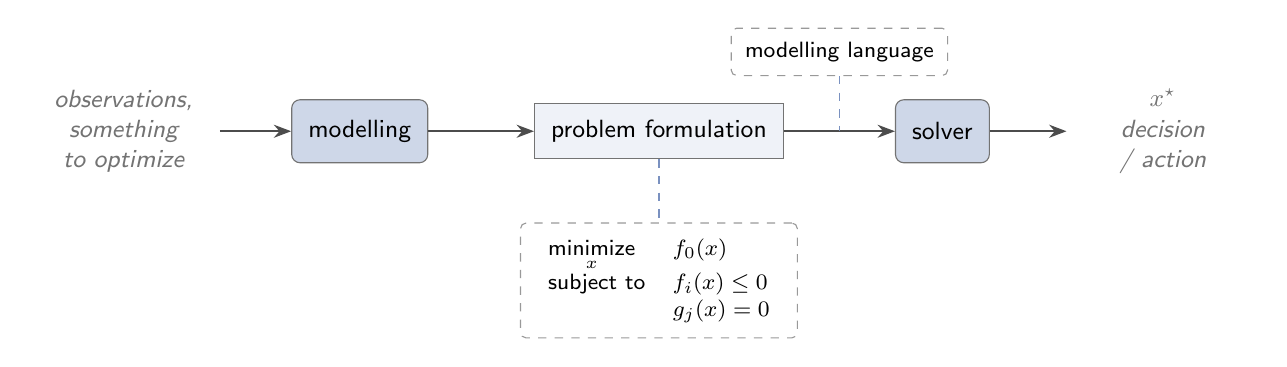
\begin{tikzpicture}
  \node[ends, text width=2.2cm] (world) at (0,0)    {observations,\\something to optimize};
  \node[proc]                   (mod)   at (3.0,0)  {modelling};
  \node[art]                    (prob)  at (6.8,0)  {problem formulation};
  \node[proc]                   (solv)  at (10.4,0) {solver};
  \node[ends, text width=2.2cm] (act)   at (13.2,0) {$\mvec{x}^\star$\\decision / action};

  \draw[flow] (world) -- (mod);
  \draw[flow] (mod)   -- (prob);
  \draw[flow] (prob)  -- node[coordinate, midway] (mid) {} (solv);
  \draw[flow] (solv)  -- (act);

  % What sits on the formulation -> solver arrow, as an annotation and not as a stage of the
  % chain. On overlay 1 with the chain: it is part of the picture, not a reveal, and bullet
  % 2 below lands on beat 2 with something already on screen to point at. Above the arrow,
  % where the band is empty -- the formulation's exbox hangs below, off the box to the left.
  \node[exbox, above=7mm of mid] (ml) {modelling language};
  \draw[zoomline] (ml.south) -- (mid);

  % Beat 2: the middle box spelled out. `visible on=' rather than \only, so the node still
  % occupies space on overlay 1 and the picture does not rescale or shift between beats.
  \node[exbox, align=center, below=8mm of prob, visible on=<2->] (ex)
    {$\begin{array}{ll}
        \underset{\mvec{x}}{\mbox{minimize}} & f_0(\mvec{x}) \\[0.5ex]
        \mbox{subject to}                    & f_i(\mvec{x}) \le 0 \\
                                             & g_j(\mvec{x}) = 0
      \end{array}$};
  \draw[zoomline, visible on=<2->] (prob.south) -- (ex.north);
\end{tikzpicture}}
\end{center}

\vspace{2ex}
\begin{itemize}\small\bul
  \item the formulation says what you want, not how to compute it
  \item<2-> {\color{polyblue}the modelling language is the bridge between the formulation
        and the solver}
\end{itemize}
\vfill
\end{frame}

% ==================================================================================
\section{Introduction}
% ==================================================================================

% --- I0b ------------------------------------------------------------------------
%  Why the deck narrows from "an optimization problem" (I0) to "a convex one" (I1).
%  Adapted from copt_talk.pdf pp. 3-4 ("Convex optimization"), essentially verbatim. The
%  thesis has nothing to lift here: there is no passage anywhere in it arguing that convex
%  problems are special -- no tractability, no global optimum, no LP/QP/SOCP/SDP taxonomy --
%  because it starts from convexity and cites Boyd and Vandenberghe. The two-beat answer
%  below is the whole reason the slide exists, so the question lands first and the answer
%  follows.
%  The display is I0's, not COPT's: COPT writes the equalities as Ax = b, and this deck
%  writes g_j(x) = 0 (see the exbox of I0). Same object on both slides, so nothing is
%  re-read. The constraint counts are left off for the same reason they are left off I0,
%  and because m is already the row count of A from I1c onwards.
%  Twin: F3a, which makes this argument for the running example.
\begin{frame}{Convex optimization}
\vspace{-1ex}
\[
  \begin{array}{ll}
    \underset{\mvec{x}}{\mbox{minimize}} & f_0(\mvec{x}) \\[0.5ex]
    \mbox{subject to}                    & f_i(\mvec{x}) \le 0 \\
                                         & g_j(\mvec{x}) = 0
  \end{array}
\]

\vspace{1ex}
\begin{itemize}\small\bul
  \item variable $\mvec{x} \in \reals^n$
  \item the equality constraints $g_j$ are affine, and $f_0$ and the $f_i$ are convex
  \item why care about convexity?
    \begin{itemize}\small
      \item<2->[--] classic answer: a local optimum is a global optimum
      \item<2->[--] modern answer: very actionable, because of reliable software
    \end{itemize}
\end{itemize}

\vfill
{\scriptsize\color{black!55} Boyd and Vandenberghe (2004).}
\end{frame}

% --- I1c ------------------------------------------------------------------------
%  The form every general-purpose solver reads. Comes before the level-2 zoom (I1), so
%  that when the zoom draws `problem -> conic form -> solver' the target of the arrow is
%  already familiar and the panel can show it as an equation rather than a phrase.
%  Source: 5-Introduction.tex:63-81 (eq:quad-conic-form, the data, the two special cases).
%  Deliberately two lines and no more. The six standard cones used to be enumerated here
%  (5-Introduction.tex:278-283); nobody retains a six-item list, the example only ever uses
%  two of them, and B2 names those two where they are actually used.
%  The QP special case -- K = R^m_+ is the nonnegative orthant -- was a bullet of its own and
%  is not coming back as one: bullet 3 below is the general form of it, and the two special
%  cases (K = R^m_+ gives a QP, P = 0 a standard conic program, 5-Introduction.tex:78-80) are
%  what to say if the floor asks which problems this covers.
%  Bullet 3 is the thesis's own sentence, 5-Introduction.tex:35-37: modern general-purpose
%  solvers have mostly moved to conic programming, which "can represent nearly every convex
%  program used in practice". The grey attribution follows I0b's pattern, and cites what the
%  thesis cites there (bental2001lectures).
\begin{frame}{Conic form}
\vspace{-1ex}
\[
  \begin{array}{ll}
    \underset{\mvec{x} \in \reals^n}{\mbox{minimize}}
      & \frac{1}{2}\mvec{x}^\top \mmat{P} \mvec{x} + \mvec{c}^\top \mvec{x} \\[0.6ex]
    \mbox{subject to} & \mvec{b} - \mmat{A}\mvec{x} \in \cone{K}
  \end{array}
\]

\vspace{1ex}
\begin{itemize}\small\bul
  \item problem data: $\mmat{P} \in \symm^n_+$,
        $\mmat{A} \in \reals^{m \times n}$, $\mvec{b} \in \reals^m$, $\mvec{c} \in \reals^n$
  \item $\cone{K} \subseteq \reals^m$ is a product of standard cones
  \item all general-purpose solvers target conic form
\end{itemize}

\vfill
{\scriptsize\color{black!55} Ben-Tal and Nemirovski (2001).}
\end{frame}

% --- I1 -------------------------------------------------------------------------
%  Zoom level 2: the problem-to-solver half of level 1, restricted to convex problems.
%  Top strip = the level-1 chain, greyed; the dashed box marks what is magnified below.
%  Titled to twin I0: `Optimization in practice' at zoom level 1, `Convex optimization in
%  practice' at level 2, so the two zoom levels are named the same way and the narrowing from
%  optimization to convex sits in the titles rather than only in the panel. Two earlier
%  titles are gone: `From convex problem to solver', which named a pipeline the strip above
%  already draws, and `Solvers', which named the two boxes at the bottom and said nothing
%  about the compilation arrow -- the half of the picture beats 3 and 4 ask about. Plain `Convex
%  optimization' is not available: it belongs to I0b and to its Example twin F3a.
%
%  Four beats: 1 the panel and what the solver runs, 2 who implements it, 3 what the panel
%  assumes about the problem, 4 what its one labelled arrow hides. The frame was going to
%  end at beat 2 with the two questions on a frame of their own; folding them in here keeps
%  the picture on screen, costs no extra frame, and is why the two standing boxes sit 24mm
%  below the panel rather than 13mm.
\begin{frame}{Convex optimization in practice}
\vfill
\begin{center}
\fitfig{%
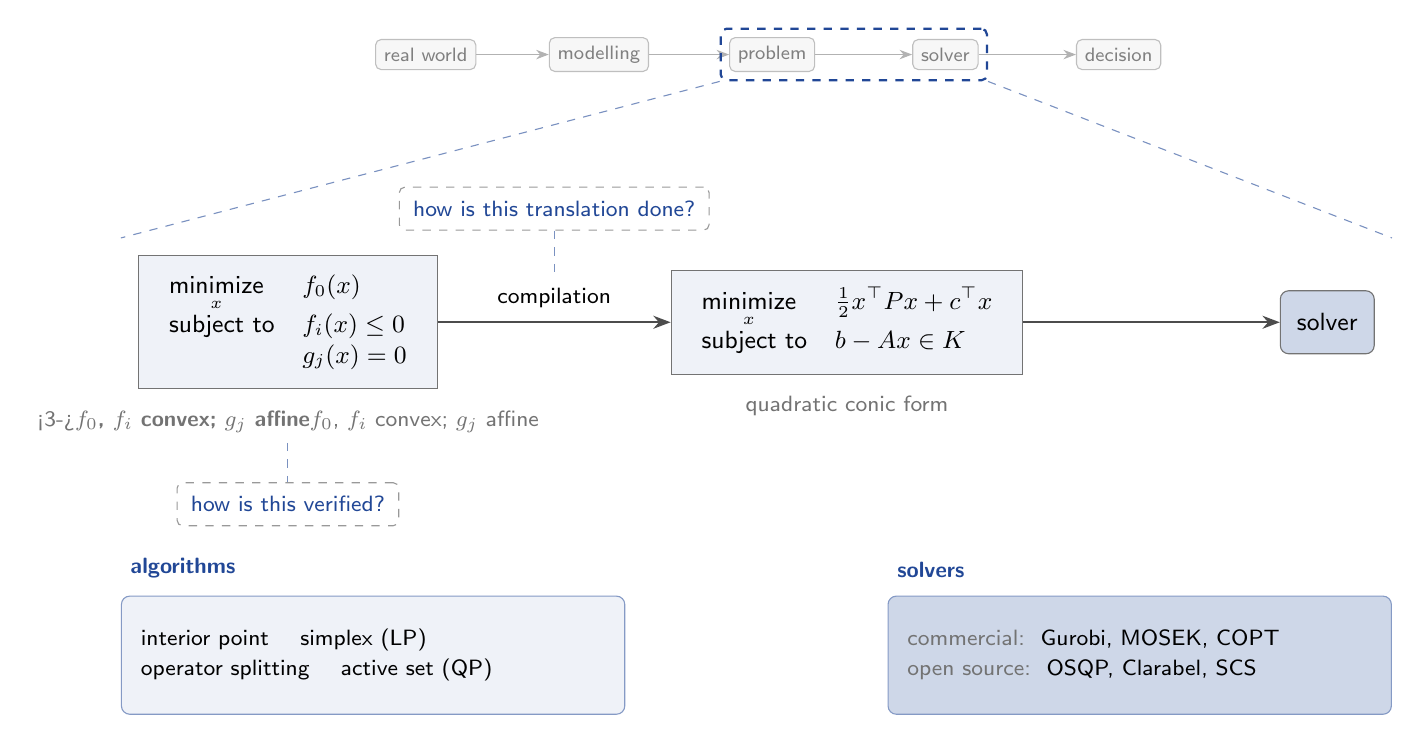
\begin{tikzpicture}
  % ---- carry-over strip (level 1, in words only) -------------------------------
  % Five boxes, matching I0's chain. The modelling language is not one of them there either:
  % on I0 it is an annotation on the problem -> solver arrow, and here it is what the
  % zoombox brackets and the panel below magnifies.
  \node[dimbox] (s1) at (1.75,0)  {real world};
  \node[dimbox] (s2) at (3.95,0)  {modelling};
  \node[dimbox] (s3) at (6.15,0)  {problem};
  \node[dimbox] (s4) at (8.35,0)  {solver};
  \node[dimbox] (s5) at (10.55,0) {decision};
  \draw[dimflow] (s1) -- (s2);  \draw[dimflow] (s2) -- (s3);
  \draw[dimflow] (s3) -- (s4);  \draw[dimflow] (s4) -- (s5);
  \node[zoombox, fit=(s3)(s4)] (zb) {};

  % ---- magnified panel ---------------------------------------------------------
  \node[art] (prob2) at (0,-3.4)
    {$\begin{array}{ll}
        \underset{\mvec{x}}{\mbox{minimize}} & f_0(\mvec{x}) \\[0.5ex]
        \mbox{subject to}                    & f_i(\mvec{x}) \le 0 \\
                                             & g_j(\mvec{x}) = 0
      \end{array}$};
  % Spelled out, not just named: the arrow is the point of the slide, and an arrow whose
  % target is a phrase says less than one whose target is the form the solver actually
  % reads. I1c, just before, named the pieces -- P, A, b, c, K -- so this is a callback to
  % an equation the room has already seen, not a new one to read.
  \node[art] (conic) at (7.1,-3.4)
    {$\begin{array}{ll}
        \underset{\mvec{x}}{\mbox{minimize}}
          & \frac{1}{2}\mvec{x}^\top \mmat{P} \mvec{x} + \mvec{c}^\top \mvec{x} \\[0.5ex]
        \mbox{subject to} & \mvec{b} - \mmat{A}\mvec{x} \in \cone{K}
      \end{array}$};
  % x = 13.2 is where the solver sits on F0 and I1b as well, so it stays put as the deck
  % zooms in. It is also the end of the chain now that x^star is gone, which leaves the
  % dashed box room to hang directly below it.
  \node[proc] (solv2) at (13.2,-3.4) {solver};

  \draw[flow] (prob2)
    -- node[edgelab, alt=<4->{text=polyblue}{}] (complab) {compilation} (conic);
  \draw[flow] (conic) -- (solv2);

  % Beats 3 and 4: the two things the panel assumes and never says, asked on the slide
  % rather than left to be spoken, and each in the mouth of the frame that answers it --
  % beat 3 hands to F1 (DCP), immediately next; beat 4 to F0 and I1b. Beat 4's question
  % therefore stays open for about a minute and a half, with F1 and F2 in between, which is
  % the point: it is what the middle of the Introduction is walking towards.
  %
  % \alt and `visible on=' throughout, never \only: every node occupies space on every
  % overlay, so the picture does not rescale between the beats. The bold on the note is
  % safe to toggle although bold is wider than upright -- the note sits under prob2, far
  % inside a bounding box the panel sets, so widening it cannot move the edges. The same
  % is NOT true in general; see B3's comment before toggling bold anywhere else.
  \node[note, alt=<3->{text=polyblue}{}, below=1.5mm of prob2] (cvxnote)
    {\alt<3->{\textbf{$f_0$, $f_i$ convex; $g_j$ affine}}%
             {$f_0$, $f_i$ convex; $g_j$ affine}};
  \node[exbox, text=polyblue, below=5mm of cvxnote, visible on=<3->] (q1)
    {how is this verified?};
  \draw[zoomline, visible on=<3->] (cvxnote.south) -- (q1.north);

  % Above the arrow rather than below it: the band between the strip and the panel is empty
  % but for the two zoom lines, which at this height have diverged past x = 2.2 and x = 11.4,
  % so a box centred over the label clears both.
  \node[exbox, text=polyblue, above=6mm of complab, visible on=<4->] (q2)
    {how is this translation done?};
  \draw[zoomline, visible on=<4->] (q2.south) -- (complab.north);
  % Names the target box the way the thesis does (5-Introduction.tex:65), and balances the
  % note under the source box on the other side of the arrow.
  \node[note, below=1.5mm of conic] {quadratic conic form};

  % ---- zoom lines from the strip down to the panel ------------------------------
  % The panel spans problem -> solver, matching the two boxes the zoombox brackets in the
  % strip: each zoom line lands on the magnified copy of the box it comes from. The two
  % standing boxes below are deliberately left out of the fit -- they fill the space under
  % the panel, they are not zoom targets.
  \node[fit=(prob2)(conic)(solv2), inner sep=6pt] (panel) {};
  \draw[zoomline] (zb.south west) -- (panel.north west);
  \draw[zoomline] (zb.south east) -- (panel.north east);

  % What a `solver' is made of, as two standing boxes filling the space under the panel,
  % in two beats: what the solver *does* first, then who implements it. No line back up to
  % the solver box -- the heading of each box says what it holds. `visible on=' rather than
  % \only, so both nodes occupy space on overlay 1 and the picture does not rescale or
  % shift between beats.
  % Lowered from -13mm to -24mm: the freed band under the left note is where the first
  % question box goes on beat 3, and the picture is width-bound (the panel spans x = -1.8
  % to 14.5, \fitfig scales to 0.98\textwidth), so the extra height costs nothing.
  \node[bigbox, anchor=north west] (methex)
    at ([yshift=-24mm]panel.south west)
    {interior point \quad simplex (LP)\\[0.4ex]
     operator splitting \quad active set (QP)};
  \node[boxtitle, above=1mm of methex.north west, anchor=south west] {algorithms};

  \node[bigbox, fill=polyblue!22, anchor=north east, visible on=<2->] (solvex)
    at ([yshift=-24mm]panel.south east)
    {{\color{black!55}commercial:}\ \ Gurobi, MOSEK, COPT\\[0.4ex]
     {\color{black!55}open source:}\ \ OSQP, Clarabel, SCS};
  \node[boxtitle, above=1mm of solvex.north west, anchor=south west,
        visible on=<2->] {solvers};
\end{tikzpicture}}
\end{center}
\vfill
\end{frame}

% --- F1 -------------------------------------------------------------------------
%  Adapted from copt_talk.pdf pp. 5-6 ("Disciplined convex programming (DCP)"), verbatim
%  but for the `sign' in bullet three, which the thesis adds (5-Introduction.tex:171-176)
%  and COPT omits.
%  Deliberately the grammar and not the rules. The composition rules themselves are already
%  in the deck twice: F3b applies them bottom-up to the running example, and the B-DCP
%  backup states them with the atom table. An introduction slide that restated them would
%  be the third telling and the least useful of the three.
%  Placed before F0, not after it: the thesis has verification gating the rewrite ("Once a
%  problem is verified to be DCP-compliant, canonicalization rewrites its functional form",
%  5-Introduction.tex:255), and the COPT talk runs in the same order. The gap I1 leaves open
%  -- its panel assumes convexity and never says who checks it -- is asked on that frame's
%  third beat, so this slide is read as the answer to a question the room has just been
%  shown. A written lead-in was tried here instead and cut. Deliberately no claim that checking convexity is
%  hard in general: the thesis makes none anywhere, and B-NONDCP carries the price of the
%  discipline (sufficient, not necessary) if it is asked for.
%  Twin: F3b.
\begin{frame}{Disciplined convex programming}
\vspace{-0.5ex}
\begin{itemize}\small\bul
  \item a grammar for specifying convex optimization problems
  \item convex and concave functions are built by combining a set of \textbf{atoms}
  \item each atom has known curvature, monotonicity in each argument, and sign
  \item simple rules specify how atoms can be composed
\end{itemize}

\vspace{2.5ex}
\onslide<2->{%
\begin{itemize}\small\bul
  \item a problem that follows the DCP rules is {\color{polyblue}convex by construction}
  \item and can be solved globally and efficiently --- in theory and in practice
\end{itemize}}

\vfill
{\scriptsize\color{black!55} Grant, Boyd and Ye (2006).}
\end{frame}

% --- F2 -------------------------------------------------------------------------
%  Adapted from copt_talk.pdf pp. 7-9 ("Modeling languages implementing DCP"), less its
%  closing beat -- `no further communication between modelling language and solver', cut
%  here and left to be spoken. The
%  analysis/synthesis split is the reason to take this slide: synthesis is canonicalization,
%  which is the deck's word for everything that follows, and I1b is titled with it -- so the
%  term has to be introduced here.
%  One addition to the COPT version: JuMP joins AMPL and GAMS, since it is the one the deck
%  actually compares against later (B-OTHERLANG, B-GAP), and `commercial' is dropped because
%  JuMP is not. What that line means -- no atom library, no canonicalization step, so a norm
%  is left to the solver or written in conic form by hand (6-Revue_litterature.tex:884-887)
%  -- is left to be spoken; it was written out here and cut. B-OTHERLANG has it in full.
%  No conic-form display: I1c showed it and the I1 panel showed it again. A third copy on
%  the same equation would be the crowding this slide is meant to avoid.
%  Twin: F3c, singular in its title because it shows one of these where this surveys them.
%
%  CVXPY on a bullet of its own, not fifth in a list of five: this slide is where the deck
%  narrows, and a name inside a survey line does not narrow anything. The bullet carries the
%  name and the colour only -- "the one this thesis targets" was written on it and cut, since
%  a line on its own in polyblue already says that, and it is the sentence to speak. The
%  frame that used to do the narrowing -- I1d, "CVXPY", with the downloads, the age and the
%  citation count --
%  sat immediately after this one and is now the backup "why CVXPY": the numbers defend the
%  choice if it is challenged, but nobody needs them to follow the talk, and I5 closes on
%  "reduce CVXPY's compilation time" with the narrowing already made here.
%  Say when the bullet is on screen that it is the one this thesis targets, and why it is the
%  one: open source, so the backend can be replaced at all -- which is what R4 claims in the
%  Conclusion.
\begin{frame}{DCP-based modelling languages}
\vspace{-0.5ex}
\begin{itemize}\small\bul
  \item \texttt{CVX} (MATLAB), \texttt{Convex.jl} (Julia), \texttt{CVXR} (R),
        \texttt{YALMIP} (MATLAB)
  \item {\color{polyblue}\cvxpy{} (Python)}
  \item \texttt{AMPL}, \texttt{GAMS} and \texttt{JuMP} do not implement DCP
  \item<2-> the two tasks of a DCP-based modelling language:
    \begin{itemize}\small
      \item<2->[--] \textbf{analysis}: verify that a high-level problem description
            follows the DCP rules
      \item<2->[--] \textbf{synthesis}: build an equivalent problem in conic form,
            called {\color{polyblue}canonicalization}
    \end{itemize}
\end{itemize}
\end{frame}

% --- I1b ------------------------------------------------------------------------
%  Zoom level 3: canonicalization itself. The accent-coloured backend arrow is the
%  only highlighted element of the two zoom slides -- that arrow is the thesis.
%
%  F0 ("Compilation") is cut, and this frame is what is left of it. F0 drew this same panel
%  generically -- model / intermediate form / P,A,b,c, at exactly these coordinates, so that
%  I1b could re-draw it with CVXPY's labels and nothing would move -- and then said in an
%  exbox what `intermediate form' means in three languages. The re-draw was the better half
%  of that gesture and it needed two frames to make; the exbox says something no other frame
%  does, so it came here and the frame went. Cut with it: F0's grey subtitle, "In DCP-based
%  languages this step is called canonicalization", which F2 already lands and this title
%  already carries. What AMPL and JuMP do instead of canonicalizing -- no atom library, so a
%  norm is left to the solver or written in conic form by hand -- is not here either; it is
%  on the backup frame "two ways to get the coefficients", where it has the evidence.
%
%  Three beats now, and the order matters: the plain chain, then the exbox (background, and
%  it dates the picture to every modelling language), then the accent arrow. The punchline
%  goes last. \fitfig is replaced by an explicit 0.76\textheight -- F0 carried the same
%  override for the same reason, the exbox hanging below the notes.
\begin{frame}{Canonicalization}
\vspace{-1ex}
\begin{center}
\adjustbox{max size={0.98\textwidth}{0.76\textheight}}{%
\begin{tikzpicture}
  % ---- carry-over strip (level 2, in words only) -------------------------------
  % The zoomed box says `canonicalization' where the level-2 strip says `compilation': this
  % is the DCP pipeline and the frame is titled with the word. The boxes are spread to 2.8
  % rather than \recallstrip's 2.4 to fit it, which moves the strip only -- the panel below
  % keeps the geometry the cut F0 shared with it.
  \node[dimbox] (t1) at (2.55,0)  {convex problem};
  \node[dimbox] (t2) at (5.35,0)  {canonicalization};
  \node[dimbox] (t3) at (8.15,0)  {conic form};
  \node[dimbox] (t4) at (10.95,0) {solver};
  \draw[dimflow] (t1) -- (t2);  \draw[dimflow] (t2) -- (t3);
  \draw[dimflow] (t3) -- (t4);
  \node[zoombox, fit=(t2)] (zb) {};

  % ---- magnified panel ---------------------------------------------------------
  % "DCP problem", not "CVXPY problem": what canonicalization takes in is a DCP-compliant
  % formulation, and F1/F2 introduced the term on the two slides just before.
  \node[art] (dcp) at (0,-3.4) {DCP problem};
  \node[art] (fconic) at (5.6,-3.4)
    {$\begin{array}{ll}
        \underset{\mvec{x}}{\mbox{minimize}} & f_0(\mvec{x};\gvec{\theta}) \\[0.5ex]
        \mbox{subject to} & h_i(\mvec{x};\gvec{\theta}) \in \cone{K}_i
      \end{array}$};
  \node[art]    (data)  at (10.5,-3.4) {$\mmat{P},\ \mmat{A},\ \mvec{b},\ \mvec{c}$};

  \draw[flow] (dcp) -- node[edgelab] {frontend} (fconic);
  % Three beats: <1> the plain chain, <2> the languages exbox, <3> the backend arrow lights
  % up and the claim lands. `alt=' / `visible on=' keep every node in the picture on every
  % overlay, so the bounding box -- and the \adjustbox scale -- do not move between beats.
  \draw[flow, alt=<3->{accent}{}] (fconic)
    -- node[edgelab, alt=<3->{text=polyblue}{}] {\alt<3->{\textbf{backend}}{backend}}
       node[font=\footnotesize, text=polyblue, midway, below=0.8mm,
            visible on=<3->] {this thesis}
    (data);

  \node[note, below=1.5mm of dcp]    {expression trees};
  % The second line is the one that matters for the thesis: the frontend does not change
  % the representation, only the content of it. What the backend walks is still a tree.
  % The third line -- f_0, h_i affine, new variables t -- was cut: B2 shows both for the
  % running example, where they can be pointed at.
  \node[note, below=1.5mm of fconic] (irn) {functional conic form\\%
                                            still expression trees};
  \node[note, below=1.5mm of data]   {explicit sparse matrices};

  % Beat 2: what "still expression trees" is an instance of. Inherited from the cut F0,
  % where it hung off the same box -- the intermediate form is the one stage of the pipeline
  % whose shape is a choice, and the three languages make three different ones. CVXPY's line
  % is the panel above, said again in a list, which is the point of the list.
  \node[exbox, below=6mm of irn, visible on=<2->] (ex)
    {\texttt{AMPL}: \texttt{.nl} file\\
     \texttt{JuMP}: MOI\\
     \cvxpy{}: expression trees};
  \draw[zoomline, visible on=<2->] (irn.south) -- (ex.north);

  % ---- zoom lines from the strip down to the panel ------------------------------
  \node[fit=(dcp)(fconic)(data), inner sep=6pt] (panel) {};
  \draw[zoomline] (zb.south west) -- (panel.north west);
  \draw[zoomline] (zb.south east) -- (panel.north east);
\end{tikzpicture}}
\end{center}
\vfill
\end{frame}

% --- I5 -------------------------------------------------------------------------
%  The last slide of the Introduction: what the backend actually does, in one picture -- a
%  forest of affine expression trees on the left, one explicit sparse [A b] on the right --
%  and the thesis's goal under it. Not a zoom level -- I1b already
%  magnified `canonicalization' into frontend/backend and lit the backend arrow, so a fourth
%  dashed-line zoom would be machinery without payload. The strip stays as a plain locator
%  with `backend' in hlbox -- the same gesture \recallstrip makes on every Example slide,
%  which is the section this hands into.
%
%  The frame used to carry the functional conic form on the left and the row/column band
%  structure as six shaded blocks on the right. Both are replaced:
%
%  1. The display is gone and the forest replaces it. What the backend walks is a tree per
%     constraint, affine by construction, and no equation on the slide said that -- the
%     audience has been told `expression trees' in a note on I1b and shown none. Deliberately
%     unlabelled nodes: this is a shape, not a parse. The Example section draws a real tree,
%     with atoms in it, three slides later (F3b), and that is where the labels belong.
%  2. The six shaded blocks are dots. The blocks said `a constraint reaches several
%     variables, a variable reappears in several constraints', which the dashed bands say on
%     their own; what they could not say is `sparse', which is the whole reason the engine
%     exists. The bands, the frame and the labels are unchanged, so the picture still reads
%     row-band = constraint, column-band = variable -- which is the link back to the forest,
%     and the sentence to speak: the forest IS this matrix, cut into rows and columns.
%
%  A companion frame was written and cut on the same pass: SC1 ("Canonicalization as sparse
%  differentiation") generalized off the running example, taking the title `Problem
%  statement' and the goal bullets while this one became `Matrix stuffing'. Two frames for
%  one idea, and the arrow below already carries the identity that was its whole payload.
%  The half of SC1 that is still not anywhere on the main deck -- P = d2f0/dx2, b = h(0),
%  c = grad f0(0), one evaluation at the origin recovering b and c, and one global Jacobian
%  per node rather than a dictionary of blocks -- is on the backup frame "two ways to get
%  the coefficients". So is the line cut from the bullets here, "it computes that Jacobian
%  sparsely, which is what the name is for": say it off the arrow when \sde{} is named.
%
%  Geometry unchanged from the shaded-block version: forest at x = 0, matrix centred at
%  x = 8.4. The figure is held to 0.38\textheight, down from 0.46, to clear three bullets.
%
%  Nothing of the method belongs on this slide. The matrix is deliberately schematic: I4
%  shows the real pattern for the example at n=5, m=8, and that slide's payload is that
%  every block is the Jacobian of the atom that produced it.
%
%  Row bands are marked with I4's `dim' double-arrows, not curly braces:
%  decorations.pathreplacing is not loaded (the preamble has pathmorphing and markings).
%
%  Sources: 5-Introduction.tex:60-77 (the conic form, one stacked x in R^n),
%           :83-86 (the cost sits in this step).
\begin{frame}{Problem statement}

% ---- locator strip: I1b's panel in words, `backend' lit -------------------------
% width 0.80\textwidth, not \recallstrip's 0.60: this strip spans 8.8 units against the
% four-box strip's 7.2, so the wider box makes the two render at the same scale. Set by
% measuring a box of this strip against one of B2's, not by the span ratio alone -- the
% two strips have different widest words, so the span ratio alone lands about 9% short.
\vspace{-2ex}
\begin{center}
\adjustbox{width=0.80\textwidth}{%
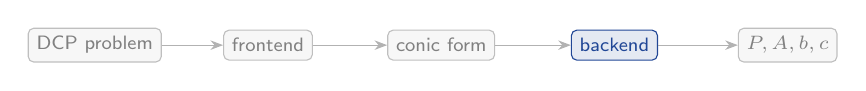
\begin{tikzpicture}
  \node[dimbox] (u1) at (0,0)   {DCP problem};
  \node[dimbox] (u2) at (2.2,0) {frontend};
  \node[dimbox] (u3) at (4.4,0) {conic form};
  \node[hlbox]  (u4) at (6.6,0) {backend};
  \node[dimbox] (u5) at (8.8,0) {$\mmat{P}, \mmat{A}, \mvec{b}, \mvec{c}$};
  \draw[dimflow] (u1) -- (u2);  \draw[dimflow] (u2) -- (u3);
  \draw[dimflow] (u3) -- (u4);  \draw[dimflow] (u4) -- (u5);
\end{tikzpicture}}
\end{center}

\vspace{0.5ex}
\begin{center}
\adjustbox{max size={0.98\textwidth}{0.38\textheight}}{%
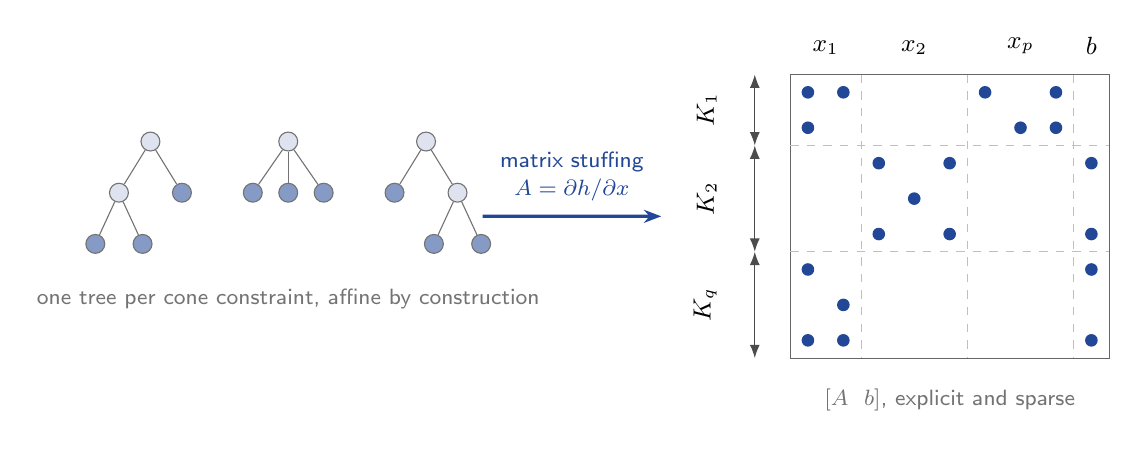
\begin{tikzpicture}
  % ---- left: a forest, one tree per cone constraint -----------------------------
  % Three trees, three row bands in the matrix opposite. Sizes and shapes differ so the
  % forest does not read as one repeated motif; nothing else about the shapes is meant.
  % Leaves are darker than internal nodes -- they are where the variables enter, and the
  % matrix opposite is grouped by variable -- but they are not labelled and do not map
  % one-for-one onto the column bands. Node radii are absolute, so they survive \adjustbox.
  \begin{scope}[
      tn/.style={circle, draw=black!55, fill=polyblue!15, inner sep=0pt, minimum size=2.4mm},
      tl/.style={circle, draw=black!55, fill=polyblue!55, inner sep=0pt, minimum size=2.4mm},
      te/.style={draw=black!55, thin}]
    % tree 1
    \node[tn] (a0) at (-1.75, 0.95) {};
    \node[tn] (a1) at (-2.15, 0.30) {};
    \node[tl] (a2) at (-1.35, 0.30) {};
    \node[tl] (a3) at (-2.45,-0.35) {};
    \node[tl] (a4) at (-1.85,-0.35) {};
    \draw[te] (a0)--(a1);  \draw[te] (a0)--(a2);
    \draw[te] (a1)--(a3);  \draw[te] (a1)--(a4);
    % tree 2
    \node[tn] (b0) at ( 0.00, 0.95) {};
    \node[tl] (b1) at (-0.45, 0.30) {};
    \node[tl] (b2) at ( 0.00, 0.30) {};
    \node[tl] (b3) at ( 0.45, 0.30) {};
    \draw[te] (b0)--(b1);  \draw[te] (b0)--(b2);  \draw[te] (b0)--(b3);
    % tree 3
    \node[tn] (c0) at ( 1.75, 0.95) {};
    \node[tl] (c1) at ( 1.35, 0.30) {};
    \node[tn] (c2) at ( 2.15, 0.30) {};
    \node[tl] (c3) at ( 1.85,-0.35) {};
    \node[tl] (c4) at ( 2.45,-0.35) {};
    \draw[te] (c0)--(c1);  \draw[te] (c0)--(c2);
    \draw[te] (c2)--(c3);  \draw[te] (c2)--(c4);
    \node[inner sep=0pt, outer sep=0pt] (forest) at (2.45,0) {};
  \end{scope}
  \node[note, align=center] at (0,-1.05)
    {one tree per cone constraint, affine by construction};

  % ---- right: the sparse [A b] the forest's entries land in ---------------------
  % Cell units inside the scope (x = y = 0.45cm), so the geometry below is in cells:
  %   columns  0-1  x_1      2-4  x_2      5-7  x_p      8  b
  %   rows     0-1  K_1      2-4  K_2      5-7  K_q
  % 9 x 8 cells = 4.05 x 3.6 cm. xshift puts its centre at x = 8.4, yshift its middle row
  % at y = 0, so the arrow from the forest runs horizontally. The cell is larger than the
  % 0.35cm this was first drawn at: the picture is width-bound by the note under the forest,
  % not height-bound, so the matrix can be grown until it reads as the other half of the
  % slide rather than as an annotation on it.
  \begin{scope}[xshift=6.375cm, yshift=1.8cm, x=0.45cm, y=0.45cm,
      dim/.style={<->, >=Latex, black!70, thin},
      lbl/.style={font=\small}]

    % The nonzeros, scattered inside six footprints: K_1 touches x_1 and x_p, K_2 touches
    % x_2 and b, K_q touches x_1 and b. Two things the picture has to say -- a constraint
    % reaches several variables, and a variable reappears in several constraints -- plus the
    % one the old shaded blocks could not: within a band it is sparse, not dense.
    % Radius 0.8mm against I4's 0.9mm, these cells being 0.45cm against I4's 0.5cm.
    \foreach \p in {(0.5,-0.5),(1.5,-0.5),(0.5,-1.5),
                    (5.5,-0.5),(7.5,-0.5),(6.5,-1.5),(7.5,-1.5),
                    (2.5,-2.5),(4.5,-2.5),(3.5,-3.5),(2.5,-4.5),(4.5,-4.5),
                    (8.5,-2.5),(8.5,-4.5),
                    (0.5,-5.5),(1.5,-6.5),(0.5,-7.5),(1.5,-7.5),
                    (8.5,-5.5),(8.5,-7.5)}
      \fill[nz] \p circle (0.8mm);

    \draw[matframe] (0,0) rectangle (9,-8);
    % one divider per variable band, and one per cone band: the grid itself is the claim
    \draw[black!25, dashed] (2,0) -- (2,-8);
    \draw[black!25, dashed] (5,0) -- (5,-8);
    \draw[black!25, dashed] (8,0) -- (8,-8);
    \draw[black!25, dashed] (0,-2) -- (9,-2);
    \draw[black!25, dashed] (0,-5) -- (9,-5);

    % ---- the column space: one band per variable -------------------------------
    \node[lbl, anchor=south] at (1,0.3)   {$\mvec{x}_1$};
    \node[lbl, anchor=south] at (3.5,0.3) {$\mvec{x}_2$};
    \node[lbl, anchor=south] at (6.5,0.3) {$\mvec{x}_p$};
    \node[lbl, anchor=south] at (8.5,0.3) {$\mvec{b}$};

    % ---- the row space: one band per cone --------------------------------------
    \draw[dim] (-1,0)  -- (-1,-2);
    \draw[dim] (-1,-2) -- (-1,-5);
    \draw[dim] (-1,-5) -- (-1,-8);
    \node[lbl, rotate=90, anchor=south] at (-1.8,-1)   {$\cone{K}_1$};
    \node[lbl, rotate=90, anchor=south] at (-1.8,-3.5) {$\cone{K}_2$};
    \node[lbl, rotate=90, anchor=south] at (-1.8,-6.5) {$\cone{K}_q$};

    \node[note, anchor=north, align=center] at (4.5,-8.6)
      {$[\mmat{A}\ \ \mvec{b}]$, explicit and sparse};

    % The arrow's landing point. Clear of the cone labels: those sit at x = -1.8 and,
    % rotated, reach about -2.7, so anything nearer puts the arrowhead on `K_2'.
    \node[inner sep=0pt, outer sep=0pt] (rpanel) at (-3.6,-4) {};
  \end{scope}

  % Two lines on the arrow, not one: `matrix stuffing' is what the step is called
  % (5-Introduction.tex:83-86) and the identity is what it is. This is the only place the
  % derivative framing appears before `A dense block at permuted positions' opens on the
  % word Jacobian, so the second line is not decoration -- say it.
  \draw[flow, accent] (forest) --
    node[edgelab, text=polyblue, align=center]
      {matrix stuffing\\[0.2ex]$\mmat{A} = \partial\mvec{h}/\partial\mvec{x}$} (rpanel);
\end{tikzpicture}}
\end{center}

\vspace{1ex}
\begin{itemize}\small\bul
  \item one stacked variable $\mvec{x} \in \reals^n$, and one full sparse matrix ---
        a row band per constraint, a column band per variable
  \item most of the compilation time is spent in this one step
  \item {\color{polyblue}the goal of this thesis is to reduce \cvxpy{}'s compilation time},
        with \sde{}, a canonicalization engine written in C
\end{itemize}
\end{frame}

% ==================================================================================
\section{Example}
% ==================================================================================

% --- F3 -------------------------------------------------------------------------
%  Opens the Example section one step earlier than the pipeline does: what the problem is
%  before it is a problem formulation. The CVXPY code moved to F3c, after the convexity
%  argument, so that the first three slides of the section are about the problem itself
%  and not about a library.
%  Stated in the Boyd/Vandenberghe idiom: no variable under `minimize' -- it is named in
%  the line below the display -- and lowercase label-prefixed fragments after it.
%  Cf. EE364a lecture 6, `Regularized approximation' (6.11) and `Scalarized problem'
%  (6.12), which is this problem: "interpretation: find good approximation Ax ~ b with
%  small x", "minimize ||Ax - b|| + gamma ||x||". That interpretation was a bullet here and
%  is now spoken -- it is the sentence anyone says while reading the display aloud, and
%  copt_talk.pdf states a problem the same way: the display, then one clipped data line.
%  The family/instance line is shortened but kept: PC0 and the whole parametric section
%  assume it.
%  Source: 5-Introduction.tex:349-364 (the problem, the data, the parameters).
\begin{frame}{Fitting with regularization}
\recallstrip[real world]{1}

\vspace{2ex}
\[
  \begin{array}{ll}
    \mbox{minimize}   & \|\mmat{F}\mvec{x}-\mvec{g}\|_2 + \mu \|\mvec{x}\|_2 \\[0.3ex]
    \mbox{subject to} & \mvec{x} \ge \zeros
  \end{array}
\]

\vspace{1ex}
\begin{itemize}\small\bul
  \item variable $\mvec{x} \in \reals^n$, data $\mmat{F} \in \reals^{m \times n}$,
        parameters $\mvec{g} \in \reals^m$ and $\mu \ge 0$
  \item one {\color{polyblue}problem family}; each value of the parameters gives a
        {\color{polyblue}problem instance}
\end{itemize}
\end{frame}

% --- F3a ------------------------------------------------------------------------
%  Twins I0b ("Convex optimization"), the slide the Introduction left to be spoken.
%  Beat 2 of the example: the convexity argument a person makes by reading the expression.
%  Deliberately informal -- its job is to be the thing F3b then does mechanically.
%  Display only, by design: the three composition steps used to be bullets below it (norm of
%  an affine map is convex; mu >= 0 scales a convex function; a sum of convex functions is
%  convex, and x >= 0 is affine) and are now spoken while pointing at the two underbraces,
%  which is what the underbraces are there for. F3b, two slides on, is the same argument
%  made mechanically, and it is the one that needs to be read rather than heard.
%  Source: 5-Introduction.tex:226-251 (the composition rules this argument uses).
\begin{frame}{Convex optimization}
\recallstrip{1}
\vfill
\[
  \underset{\mvec{x} \ge \zeros}{\mbox{minimize}}\quad
  \underbrace{\|\mmat{F}\mvec{x}-\mvec{g}\|_2}_{\text{\normalfont\footnotesize convex}}
  \; + \;
  \underbrace{\mu \|\mvec{x}\|_2}_{\text{\normalfont\footnotesize convex}}
\]
\vfill
\end{frame}

% --- F3c ------------------------------------------------------------------------
%  Twins F2 ("DCP-based modelling languages"); singular in the title because this shows
%  one of them where F2 surveys the family.
%  Beat 3: the same problem handed to a modelling language, placed after the convexity
%  argument so that the code is read as a transcription of something already understood.
%  It also sets up F3b and F3e: `nonneg=True' is what makes the DCP check pass, and F3e's
%  `mul' row is where that is spelled out --
%  which is why the second surviving bullet stays. The first bullet -- "the problem is
%  written the way it is stated: atoms and operators, not matrices" -- came off: it is a
%  reading of the listing directly above it, and is spoken while the code is on screen.
%  Source: lst:cvxpy-example (5-Introduction.tex:365-374), imports included, so the slide
%  and the thesis listing show the same code.
%  `mypython' (listing_defs.tex:39) rather than plain Python: it colours the CVXPY and NumPy
%  names green and the keywords magenta, which is what makes `Parameter' and `Variable'
%  findable while the bullets below talk about them.
%  [fragile] is required: the frame carries an lstlisting.
\begin{frame}[fragile]{A DCP-based modelling language}
\recallstrip[\cvxpy{} problem]{1}

\begin{center}
\begin{minipage}{0.80\textwidth}
% aboveskip/belowskip override mypython's 1em: the imports and the blank line cost three
% lines, and without this the frame pushes the recall strip into the title.
\begin{lstlisting}[language=mypython, basicstyle=\ttfamily\small,
                   aboveskip=0.4em, belowskip=0.4em]
import cvxpy as cp
import numpy as np

F  = np.random.randn(m, n)
x  = cp.Variable(n)
g  = cp.Parameter(m)
mu = cp.Parameter(nonneg=True)

objective = cp.Minimize(
    cp.norm(F @ x - g) + mu * cp.norm(x))
prob = cp.Problem(objective, [x >= 0])
\end{lstlisting}
\end{minipage}
\end{center}

\vspace{1ex}
\begin{itemize}\small\bul
  \item \texttt{Parameter} marks what changes between solves; \texttt{Variable} what is
        solved for
  \item nothing here says how to solve it, or that it is convex
\end{itemize}
\end{frame}

% --- F3b ------------------------------------------------------------------------
%  Twins F1 ("Disciplined convex programming").
%  Beat 3: the same argument made mechanically, bottom-up over the tree. The tree is
%  fig:dcp-expression-tree (5-Introduction.tex:382-410) with \annotatedop dropped --
%  \annotatedop reserves a \phantom copy of its second argument, doubling every node's
%  width -- and the curvature carried by node fill instead, so no node grows.
%  The mu >= 0 point is the payoff of `nonneg=True' on the previous slide.
\begin{frame}{Disciplined convex programming}
\recallstrip[DCP problem]{1}
\vspace{-1ex}
{\small \cvxpy{} stores the objective and each constraint as an expression tree:}
\vspace{-1ex}
\begin{center}
% Compacted rather than capped: the sibling and level distances below are tight enough
% that \fitfig no longer has to shrink the picture, so the nodes read larger on screen
% than they did inside a 0.50\textheight box with white space in it.
\fitfig{%
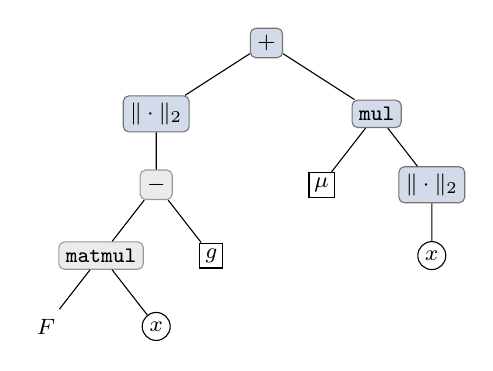
\begin{tikzpicture}[level 1/.style={sibling distance=28mm},
                    level 2/.style={sibling distance=14mm},
                    level distance=9mm,
                    every node/.style={font=\footnotesize},
                    cvx/.style={fill=polyblue!20, draw=black!55, rounded corners=2pt,
                                inner sep=2.5pt},
                    aff/.style={fill=black!8, draw=black!40, rounded corners=2pt,
                                inner sep=2.5pt}]
  \node[cvx] {$+$}
    child {node[cvx] {$\|\cdot\|_2$}
      child {node[aff] {$-$}
        child {node[aff] {\texttt{matmul}}
          child {node {$\mmat{F}$}}
          child {node[circle, draw, inner sep=1.5pt] {$\mvec{x}$}} }
        child {node[draw, inner sep=2pt] {$\mvec{g}$}} } }
    child {node[cvx] {\texttt{mul}}
      child {node[draw, inner sep=2pt] {$\mu$}}
      child {node[cvx] {$\|\cdot\|_2$}
        child {node[circle, draw, inner sep=1.5pt] {$\mvec{x}$}} } };
\end{tikzpicture}}

\vspace{0.5ex}
{\footnotesize\color{black!55}
\tikz[baseline=-0.5ex]\node[fill=polyblue!20, draw=black!55, rounded corners=1pt,
      minimum width=3mm, minimum height=2.4mm, inner sep=0pt]{};\ convex \quad
\tikz[baseline=-0.5ex]\node[fill=black!8, draw=black!40, rounded corners=1pt,
      minimum width=3mm, minimum height=2.4mm, inner sep=0pt]{};\ affine \quad
$\bigcirc$ variable \quad $\square$ parameter}
\end{center}

\end{frame}

% --- F3e ------------------------------------------------------------------------
%  Where the colours on the previous slide came from. F3b tints every node convex or affine
%  and does not say who decided; this is the answer, and it is the only slide in the main
%  deck that shows the atom library as a library rather than naming it (F1, bullet 2).
%
%  Placed after the tree rather than before it, deliberately: the tinted tree is what makes
%  the question `how did it know?' land, and a table read before there is a question to
%  answer is a table nobody reads. The cost is that F3b is, for one slide, a picture whose
%  mechanism is still pending -- which is the trade taken.
%
%  The rows are tab:atoms of the thesis (5-Introduction.tex:186-196), six of its nine: sum,
%  abs, square and sqrt are there to show a library with all three curvatures and both
%  monotonicity verdicts in it, and `norm' and `mul' are the two this problem actually uses,
%  marked so the tree of the previous slide can be checked against them row by row.
%  `mul' is not a row of tab:atoms -- the thesis lists it nowhere, because scalar
%  multiplication is not interesting on its own. It is here because it is the row that makes
%  `nonneg=True' on F3c matter: mul is affine either way, but only a nonnegative multiplier
%  makes it non-decreasing, which is the clause the composition rule needs for mu*norm(x).
%
%  The marking is a polyblue triangle in a narrow leading column plus a polyblue atom name,
%  not \rowcolor: colortbl is not loaded, and the deck colours text rather than cells
%  everywhere else.
%
%  Only the two clauses this problem uses are stated below the table. The full three-case
%  composition rule, the DCP-compliance conditions and the sufficient-not-necessary caveat
%  are the backup frame "the DCP rules", which keeps tab:atoms' own five-row selection --
%  that frame answers "what exactly are the rules?", this one answers "what is an atom?".
\begin{frame}{Atoms}
\recallstrip[DCP problem]{1}
{\small Every atom declares its curvature, its monotonicity in each argument, and the sign of
its output:}

\vspace{1.5ex}
\begin{center}\footnotesize
\setlength{\tabcolsep}{5pt}
\begin{tabular}{@{}c l l l l l@{}}
\toprule
 & Atom & Definition & Curvature & Monotonicity & Sign \\
\midrule
 & \texttt{sum}    & $\textstyle\sum_i x_i$ & affine  & non-decreasing & any \\
 & \texttt{abs}    & $|x|$                  & convex  & unknown        & nonnegative \\
 & \texttt{square} & $x^2$                  & convex  & unknown        & nonnegative \\
 & \texttt{sqrt}   & $\sqrt{x}$             & concave & non-decreasing & nonnegative \\
{\color{polyblue}$\blacktriangleright$} & {\color{polyblue}\texttt{norm}}
   & $\|\mvec{x}\|_2$ & convex & unknown & nonnegative \\
{\color{polyblue}$\blacktriangleright$} & {\color{polyblue}\texttt{mul}}
   & $\mu\mvec{x},\ \mu \ge 0$ & affine & non-decreasing & any \\
\bottomrule
\end{tabular}
\end{center}

\vspace{2ex}
\begin{center}\small
{\color{polyblue}convex $\circ$ affine is convex}, so $\|\mmat{F}\mvec{x}-\mvec{g}\|_2$ is;
and $\mu \ge 0$ makes \texttt{mul} non-decreasing, so $\mu\|\mvec{x}\|_2$ is too.\\[0.5ex]
{\color{black!55}\footnotesize Which is what \texttt{cp.Parameter(nonneg=True)} was for.}
\end{center}
\end{frame}

% --- B2 -------------------------------------------------------------------------
%  Twins the frontend half of I1b ("Canonicalization: frontend and backend"). The example
%  is finer than the Introduction here: I1b draws both arrows on one slide, this section
%  gives each its own, which is what the paired titles say.
%  eq:graph, 5-Introduction.tex:420-431, and the sentence that follows it at :432-438.
%  Two things came off the bullets and are spoken: the cone written out as the product
%  R_+^n x K_soc,m+1 x K_soc,n+1 -- which reads off the three constraint lines of the
%  display, and which I4 labels again on its row space -- and "one affine expression tree
%  per constraint".
\begin{frame}{Canonicalization: the frontend}
\recallstrip{2}
\vspace{-1ex}
\[
  \begin{array}{ll}
    \underset{t_1,\, t_2,\, \mvec{x}}{\mbox{minimize}} & t_1 + \mu t_2 \\[0.4ex]
    \mbox{subject to}
      & \mvec{x} \ge \zeros \\
      & (t_1,\ \mmat{F}\mvec{x} - \mvec{g}) \in \cone{K}_{\mathrm{soc},\, m+1} \\
      & (t_2,\ \mvec{x}) \in \cone{K}_{\mathrm{soc},\, n+1}
  \end{array}
\]

\vspace{1ex}
\begin{itemize}\small\bul
  \item the norms become epigraph variables $t_1$, $t_2$, one cone constraint each
  \item every constraint is a cone membership, and {\color{polyblue}every expression left
        is affine in $(t_1, t_2, \mvec{x})$}
\end{itemize}
\end{frame}

% --- B3 -------------------------------------------------------------------------
%  Twins the backend half of I1b, and the panel of I5 ("Problem statement"): this is what
%  matrix stuffing produced for this problem.
%  The stuffed data for the example. Source: fig:matrix-stuffing root nodes,
%  6-Revue_litterature.tex:221-225 (c) and :258-268 ([A b]); column order z = (t1, t2, x)
%  is fixed at 6-Revue_litterature.tex:174-182. The sign note is the figure's caption,
%  6-Revue_litterature.tex:310-311. It was a bullet on beat 1 and came off, and the grey line
%  on SC1 that used to repeat it went with that frame -- so the sign convention is nowhere on
%  the deck now. Say it here, once, while the minus signs are on screen; the backup frame
%  "two ways to get the coefficients" is where to go if it is pressed.
%  P is genuinely absent here: the objective canonicalized to t1 + mu*t2, which is linear.
%
%  Beat 2 was a separate frame, B4 "A parameter change" (the claim of
%  5-Introduction.tex:134-137: a parameter changes the values of the problem data but not
%  their structure). The two frames drew the same matrix twice, so beat 2 now says what B4
%  said while the picture holds still -- the gesture I0, I1 and I1b make with `visible on='.
%  \only rather than \alt: the lead line and the bullets differ between the beats too.
%  The \boldsymbol beat 2 used to put on mu and -g is dropped: bold is wider than upright, so
%  \fitfig would rescale the whole figure between the beats. Against a matrix that is grey
%  everywhere else, the colour alone carries it.
\begin{frame}{Canonicalization: the backend}
\recallstrip{3}
\vspace{-1ex}
\only<1>{{\small Stack the variables as $\mvec{z} = (t_1, t_2, \mvec{x})$ and the data falls
out:}}%
\only<2>{{\small The parameters are $\mvec{g}$ and $\mu$. Everything else is fixed for the
whole problem family:}}

\vspace{1ex}
\begin{center}
\only<1>{\fitfig{%
$\mvec{c}^\top =
\begin{blockarray}{ccc}
 t_1 & t_2 & \mvec{x} \\
\begin{block}{[ccc]}
 1 & \mu & \plotzero \\
\end{block}
\end{blockarray}
\qquad
[\mmat{A}\ \ \mvec{b}] =
\begin{blockarray}{cccc}
 t_1 & t_2 & \mvec{x} & \mvec{b} \\
\begin{block}{[cccc]}
 \plotzero & \plotzero & -\mmat{I} & \plotzero \\
 -1        & \plotzero & \plotzero & \plotzero \\
 \plotzero & \plotzero & -\mmat{F} & -\mvec{g} \\
 \plotzero & -1        & \plotzero & \plotzero \\
 \plotzero & \plotzero & -\mmat{I} & \plotzero \\
\end{block}
\end{blockarray}$}}%
\only<2>{\fitfig{%
$\mvec{c}^\top =
\begin{blockarray}{ccc}
 t_1 & t_2 & \mvec{x} \\
\begin{block}{[ccc]}
 \color{black!35}1 & \color{polyblue}\mu & \color{black!35}\plotzero \\
\end{block}
\end{blockarray}
\qquad
[\mmat{A}\ \ \mvec{b}] =
\begin{blockarray}{cccc}
 t_1 & t_2 & \mvec{x} & \mvec{b} \\
\begin{block}{[cccc]}
 \color{black!35}\plotzero & \color{black!35}\plotzero & \color{black!35}-\mmat{I} & \color{black!35}\plotzero \\
 \color{black!35}-1        & \color{black!35}\plotzero & \color{black!35}\plotzero & \color{black!35}\plotzero \\
 \color{black!35}\plotzero & \color{black!35}\plotzero & \color{black!35}-\mmat{F} & \color{polyblue}-\mvec{g} \\
 \color{black!35}\plotzero & \color{black!35}-1        & \color{black!35}\plotzero & \color{black!35}\plotzero \\
 \color{black!35}\plotzero & \color{black!35}\plotzero & \color{black!35}-\mmat{I} & \color{black!35}\plotzero \\
\end{block}
\end{blockarray}$}}
\end{center}

\only<1>{%
\vspace{0.5ex}
\begin{itemize}\footnotesize\bul
  \item the five row blocks are the three cone constraints, in the order
        $\reals_+^n$, $\cone{K}_{\mathrm{soc},m+1}$, $\cone{K}_{\mathrm{soc},n+1}$
  \item {\color{polyblue}$\mmat{P} = \zeros$ here}: the objective is linear
\end{itemize}}%
\only<2>{%
\vspace{1.5ex}
\begin{itemize}\footnotesize\bul
  \item $\mu$ lands in one entry of $\mvec{c}$; $\mvec{g}$ lands in one block of $\mvec{b}$
  \item every other entry --- the signs, the identities, the data $\mmat{F}$ --- is the same
        at every solve
  \item {\color{polyblue}and the \emph{positions} never move at all}
\end{itemize}}
\end{frame}

% --- I4 -------------------------------------------------------------------------
%  Last slide of the Example section, and the second of its two data slides: B3 gives the
%  data and, on its second beat, what a parameter touches; this one gives the structure that
%  never moves. Its closing
%  line hands into the method, which opens the next section on SC0, the storage format.
%
%  The pattern is the running example's own [A b], not a synthetic one: the blocks of B3
%  ("The problem data") drawn at n = 5, m = 8. Every feature on the slide is therefore
%  something the audience has already seen symbolically.
%  Sources: 6-Revue_litterature.tex:258-268 ([A b]), :174-182 (column order z = (t1,t2,x)),
%           7-Theme1.tex:149-156 (the Jacobian of Bx places a dense block at the columns
%           of x), 6-Revue_litterature.tex:493-504 (CVXPY's backends store dense constant
%           data as sparse matrices).
%
%  Geometry: 8 columns x 20 rows of cells, x=y=0.5cm, origin at the top-left corner of the
%  matrix, rows growing downwards (negative y).
%    columns  0      t1
%             1      t2
%             2-6    x            (n = 5)
%             7      b
%    rows     0-4    -I on the columns of x          x >= 0,  n rows
%             5      -1 at t1                        SOC m+1, first row
%             6-13   -F on x, -g on b                SOC m+1, m rows
%             14     -1 at t2                        SOC n+1, first row
%             15-19  -I on the columns of x          SOC n+1, n rows
%  The matrix is necessarily taller than it is wide (2n+m+2 rows, n+2 columns) for every n
%  and m, so it is height-bound whatever width it is given; n and m are kept small for
%  exactly that reason, the row count is what sets how large the cells can be.
%  It used to sit in a 0.46\textwidth column with a two-bullet reading of it on the right --
%  a dense block, two identity diagonals, two lone entries; none of it discovered, every
%  block the Jacobian of the atom that produced it -- closing on "a generic sparse format
%  stores all of it as unrelated (row, column, value) triples". All three lines are an
%  inventory of what the picture already shows, so they are spoken and the matrix takes the
%  whole frame instead. The last of them is the hand-off to SC0, which opens on CSR, and is
%  the one to be sure of saying.
\begin{frame}{Structure in the problem data}
\recallstrip{3}
% The caption lives under the matrix rather than above it: the picture is height-bound
% (2n+m+2 rows against n+2 columns), so every line of text above it shrinks the cells.
% \centering inside a group rather than the center environment, for the same reason: center
% adds a \topsep above and below, and each of those comes straight off the cell size.
{\centering
\adjustbox{max size={0.92\textwidth}{0.74\textheight}}{%
% Drawn at 0.5cm cells, larger than the picture needs: adjustbox's `max size' only ever
% shrinks, so at its natural size the cap did nothing and the matrix could not grow.
% Over-sizing it here puts the cap in charge of the final size.
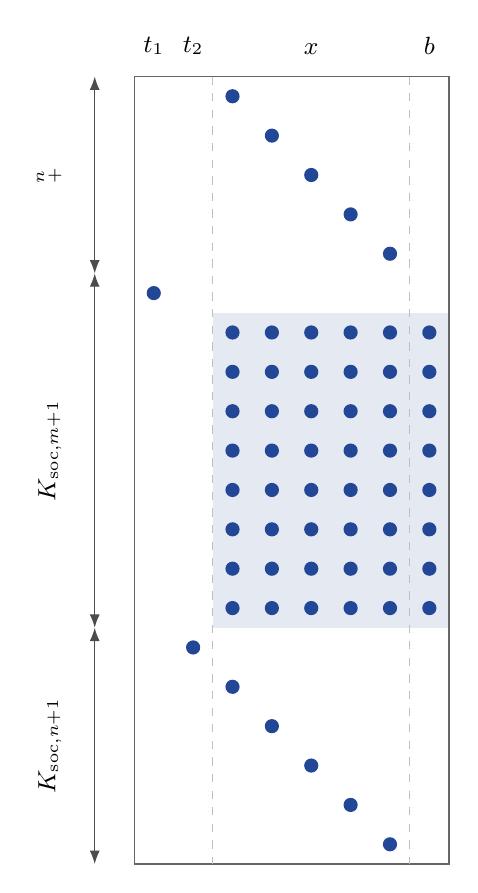
\begin{tikzpicture}[x=0.5cm, y=0.5cm,
    dim/.style={<->, >=Latex, black!70, thin},
    lbl/.style={font=\small}]

  % ---- block shading, behind the dots ------------------------------------------
  \fill[polyblue!12] (2,-6) rectangle (7,-14);      % -F
  \fill[polyblue!12] (7,-6) rectangle (8,-14);      % -g

  % ---- the matrix ---------------------------------------------------------------
  \draw[matframe] (0,0) rectangle (8,-20);
  \draw[black!25, dashed] (2,0) -- (2,-20);
  \draw[black!25, dashed] (7,0) -- (7,-20);

  % -I on the columns of x, from x >= 0
  \foreach \r in {0,...,4} \fill[nz] (2+\r+0.5,-\r-0.5) circle (0.9mm);
  % the epigraph variable t1
  \fill[nz] (0.5,-5.5) circle (0.9mm);
  % -F, dense, and -g beside it
  \foreach \r in {6,...,13} {
    \foreach \c in {2,...,6} \fill[nz] (\c+0.5,-\r-0.5) circle (0.9mm);
    \fill[nz] (7.5,-\r-0.5) circle (0.9mm);
  }
  % the epigraph variable t2
  \fill[nz] (1.5,-14.5) circle (0.9mm);
  % -I on the columns of x again, from the second cone
  \foreach \r in {0,...,4} \fill[nz] (2+\r+0.5,-15-\r-0.5) circle (0.9mm);

  % ---- the column space ---------------------------------------------------------
  \node[lbl, anchor=south] at (0.5,0.3) {$t_1$};
  \node[lbl, anchor=south] at (1.5,0.3) {$t_2$};
  \node[lbl, anchor=south] at (4.5,0.3) {$\mvec{x}$};
  \node[lbl, anchor=south] at (7.5,0.3) {$\mvec{b}$};

  % ---- the row space: one band per cone -----------------------------------------
  \draw[dim] (-1,0)   -- (-1,-5);
  \draw[dim] (-1,-5)  -- (-1,-14);
  \draw[dim] (-1,-14) -- (-1,-20);
  \node[lbl, rotate=90, anchor=south] at (-1.6,-2.5)  {$\reals_+^n$};
  \node[lbl, rotate=90, anchor=south] at (-1.6,-9.5)  {$\cone{K}_{\mathrm{soc},m+1}$};
  \node[lbl, rotate=90, anchor=south] at (-1.6,-17)   {$\cone{K}_{\mathrm{soc},n+1}$};
\end{tikzpicture}}

\vspace{0.5ex}
{\footnotesize $[\mmat{A}\ \ \mvec{b}]$ for the example, at $n = 5$ and $m = 8$}
\par}
\end{frame}

% ==================================================================================
\section{Single canonicalization}
% ==================================================================================

% --- SC0 --------------------------------------------------------------------------
%  Opens the contributions section with the storage format everything after it is expressed
%  in: SC2's (X, r, c) triple is a dense block at permuted positions *against* CSR, SC3's
%  kernels dispatch on it, and the backup slide "addition is where the dense path stops"
%  turns on CSR views sharing idxptr/cols without copying vals. None of those read without
%  CSR on the board first.
%
%  Matrix and listing are the thesis's own, copied rather than redrawn: S is
%  5-Introduction.tex:759-765 (eq:sparse-matrix) and the arrays are lst:csr-format at
%  :786-790, down to the spacing that puts each idxptr entry above the start of its row in
%  cols. Nothing is shaded or coloured -- the alignment is what ties a row to its slice, and
%  a reader who has the document open sees the same two objects there.
%
%  The running example's [A b] of I4 cannot play this part: at n = 5, m = 8 it has sixty
%  nonzeros and the arrays would not fit on a slide.
%
%  [fragile] is required: the frame carries an lstlisting.
%
%  Sources: 5-Introduction.tex:748-797 (COO, CSR, and why rows are contiguous),
%           7-Theme1.tex:130-146 (CSR over CSC, and the split between the symbolic pass
%           writing idxptr/cols and the numeric pass writing vals).
\begin{frame}[fragile]{Compressed sparse row}
% The section's punchline, said once, before any mechanism. It sits here rather than on a
% frame of its own: a `Contributions' frame existed (I6, d3ab9fd) and was cut on purpose in
% ac78a2c so that the Example answers the problem statement instead of preceding a list of
% answers. The line also gives this slide its reason for opening the section -- CSR is the
% format the new classes depart from, not a contribution in itself.
\vspace{-0.5ex}
{\small {\color{polyblue}New matrix classes for the structure the problem data already has,
and kernels that dispatch on them.} Starting from what everything is stored in today:}

\vfill
\begin{columns}[c,onlytextwidth]
\begin{column}{0.30\textwidth}
\centering
\[
  \mmat{S} = \begin{bmatrix}
    0 & 1 & 0 & 0\\
    2 & 0 & 3 & 4\\
    0 & 5 & 6 & 0\\
  \end{bmatrix}
\]
\end{column}
\begin{column}{0.66\textwidth}
% keepspaces/columns=fixed: the listing's alignment is the content here, so the spacing of
% idxptr must survive verbatim.
\begin{lstlisting}[language=C, basicstyle=\ttfamily\small, columns=fixed, keepspaces=true,
                   aboveskip=0.4em, belowskip=0.4em]
int  idxptr[] = {0,  1,          4,      6};
int    cols[] = {1,  0,  2,  3,  1,  2};
double vals[] = {1,  2,  3,  4,  5,  6};
\end{lstlisting}
\end{column}
\end{columns}

\vspace{2ex}
\begin{itemize}\small\bul
  \item row $i$ is the contiguous slice
        \texttt{vals[idxptr[i]:idxptr[i+1]]} --- reached in constant time, so a slice of
        rows is {\color{polyblue}a view, not a copy}
\end{itemize}
\vfill
\end{frame}
% --- SC2 --------------------------------------------------------------------------
%  The thesis's own figure, fig:permuted-dense at 7-Theme1.tex:206-272, put on the slide
%  rather than redrawn on the running example. An earlier version of this frame lit the -F
%  block of I4's [A b] instead, on the argument that the deck never introduces a matrix
%  called B; that version is gone by preference -- the thesis figure is sized for teaching
%  (4 x 10 with a 4 x 2 block) where the running example is not (at n = 5, m = 8 the block
%  is 8 x 5 in a 13-column matrix, which cannot be written out entry by entry), and the row
%  tints carry the correspondence between A and X in a way the dot picture cannot. The one
%  This frame now opens the section's argument, with SC1 ("Canonicalization as sparse
%  differentiation") cut: the word Jacobian arrives here for the first time in the section,
%  and what licenses it is the accent arrow of I5, which carries A = dh/dz.
%  line under A used to do the bridging the old picture did structurally -- "of a problem
%  with ten variable entries, the -F block of the last slide, in miniature" -- and is now a
%  gesture and a sentence: the -F block is still on screen one slide back if it is needed.
%  The tail of beat 2's first bullet went the same way: "and the global matrix is never
%  formed" is the claim SC3 used to repeat as "no selector matrix is ever formed", and it is
%  now said once, out loud, on whichever of the two slides it comes up.
%
%  Colours are the thesis's LOCAL values (7-Theme1.tex:203-206: blue!12, green!16,
%  orange!22, purple!14), not the deck's preamble pdRowA..D, which are the same hues two to
%  three steps stronger and read as loud on a projector. They are overridden here rather
%  than in the preamble so the permuted-dense figures elsewhere in the deck keep their
%  values.
%
%  Beat 1 is what the Jacobian looks like, beat 2 what is stored. \onslide, not \only: it
%  reserves beat 2's space, so the top display does not move between the beats.
\colorlet{pdRowA}{blue!12}
\colorlet{pdRowB}{green!16!white}
\colorlet{pdRowC}{orange!22!white}
\colorlet{pdRowD}{purple!14!white}
\begin{frame}{A dense block at permuted positions}
\vspace{-1ex}
{\footnotesize The Jacobian of $\mmat{B}\mvec{x}$ with dense
$\mmat{B} \in \reals^{4\times2}$, for $\mvec{x}$ at columns $(4,5)$:}

% NOT inside \fitfig: nicematrix places its \CodeBefore panels with absolute coordinates,
% which a scalebox displaces -- inside \fitfig the row tints leave the matrix and run the
% height of the frame. The size is set with \small instead, and the display fits at that.
\vspace{0.5ex}
\begin{center}
{\small
$\mmat{A} =
\begin{pNiceMatrix}[margin]
\CodeBefore
  \rectanglecolor{pdRowA}{1-5}{1-6}
  \rectanglecolor{pdRowB}{2-5}{2-6}
  \rectanglecolor{pdRowC}{3-5}{3-6}
  \rectanglecolor{pdRowD}{4-5}{4-6}
\Body
\cdot & \cdot & \cdot & \cdot & b_{00} & b_{01} & \cdot & \cdot & \cdot & \cdot \\
\cdot & \cdot & \cdot & \cdot & b_{10} & b_{11} & \cdot & \cdot & \cdot & \cdot \\
\cdot & \cdot & \cdot & \cdot & b_{20} & b_{21} & \cdot & \cdot & \cdot & \cdot \\
\cdot & \cdot & \cdot & \cdot & b_{30} & b_{31} & \cdot & \cdot & \cdot & \cdot
\end{pNiceMatrix}
\qquad
\mmat{X} =
\begin{pNiceMatrix}[margin]
\CodeBefore
  \rectanglecolor{pdRowA}{1-1}{1-2}
  \rectanglecolor{pdRowB}{2-1}{2-2}
  \rectanglecolor{pdRowC}{3-1}{3-2}
  \rectanglecolor{pdRowD}{4-1}{4-2}
\Body
b_{00} & b_{01} \\
b_{10} & b_{11} \\
b_{20} & b_{21} \\
b_{30} & b_{31}
\end{pNiceMatrix}$}
\end{center}

\vspace{0.5ex}
\begin{center}
$\mvec{r} = (0,1,2,3), \qquad \mvec{c} = (4,5)$
\end{center}

\onslide<2->{%
\vspace{1.5ex}
\begin{center}
$\mmat{A} = \mmat{S}_r^\top \mmat{X} \mmat{S}_c$, \qquad $A_{r_i,\, c_j} = X_{ij}$
\end{center}

\vspace{0.5ex}
\begin{itemize}\footnotesize\bul
  \item store the triple $(\mmat{X}, \mvec{r}, \mvec{c})$: one index per row and per column,
        not one per entry
  \item {\color{polyblue}the storage does not depend on the global dimensions $m$ and $n$}
\end{itemize}}
\end{frame}

% --- SC3 --------------------------------------------------------------------------
%  The payoff, and where BLAS lands: carried by the mechanism, not by a benchmark.
%
%  The identity B'A = S_cB' X_B' (S_rB S_rA') X_A S_cA (eq:pd-product, 7-Theme1.tex:508) was
%  beat 1 and is CUT: five selector matrices and a nested underbrace is the densest formula
%  the deck ever showed, and what it says out loud is the three bullets that replaced it --
%  intersect the row vectors, one dgemm, nothing formed. It is on the backup frame "which
%  kernel runs on which pair" for anyone who wants to see it written down. SC2 still carries
%  A = S_r' X S_c, which is the definition and reads in one line.
%
%  Two beats. Beat 1 is the mechanism in words; beat 2 is dispatch, as a 2 x 2 grid in place
%  of the two bullets that used to state the same thing in prose. The grid is what is left
%  of the 3 x 3 kernel-dispatch table that sat here before: its sPD row and column are gone,
%  because the deck never names that representation (SC2 describes it in passing without
%  christening it), and with them go six cells and half the legend. What remains is the only
%  claim the slide needs -- the dense form is absorbing, and only sparse against sparse
%  stays sparse. The full 3 x 3 with sPD is the backup frame "which kernel runs on which
%  pair", below \appendix, where a question can reach it.
%
%  \onslide, not \only: beat 2's space is reserved, so the identity does not move.
%  Two tints only, both quiet: polyblue!10 for the cells that come out dense, black!6 for
%  the one that does not. The old table's four-colour legend was the other half of what made
%  it slow to read, and no legend replaces it -- the line under the grid says what the tint
%  means, so there is one thing to read rather than two.
%  Sources: 7-Theme1.tex:508-522 (eq:pd-product and the two-pass sentence),
%           7-Theme1.tex:440-503 (fig:kernel-dispatch and the kernel families).
\begin{frame}{Closed under the operations we need}
\vspace{1ex}
{\small The product of two permuted dense matrices
$\mmat{A} = (\mmat{X}_A, \mvec{r}_A, \mvec{c}_A)$ and
$\mmat{B} = (\mmat{X}_B, \mvec{r}_B, \mvec{c}_B)$ is another one:}

\vspace{1.5ex}
\begin{itemize}\small\bul
  \item the symbolic pass {\color{polyblue}intersects $\mvec{r}_B$ with $\mvec{r}_A$} ---
        both sorted, so one walk
  \item the numeric pass multiplies the blocks with {\color{polyblue}one \texttt{dgemm}}
\end{itemize}

\onslide<2->{%
\vspace{2ex}
\begin{center}
\fitfig{%
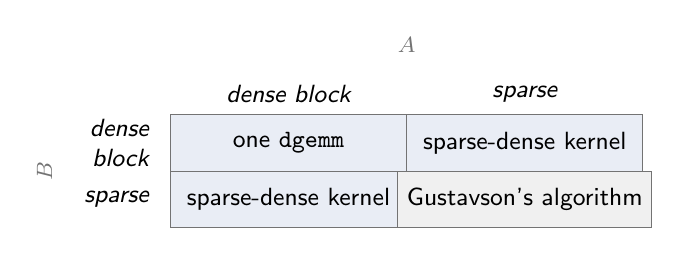
\begin{tikzpicture}[
  cell/.style={draw=black!55, minimum width=3.0cm, minimum height=0.72cm,
               font=\small, anchor=center},
  densec/.style={cell, fill=polyblue!10},
  sparsec/.style={cell, fill=black!6},
  hdr/.style={font=\small\itshape, anchor=center},
]
\def\dx{3.0}
\def\dy{0.72}
\node[font=\footnotesize, text=black!55] at (\dx/2, 1.25) {$\mmat{A}$};
\node[hdr] at (0, 0.62)   {dense block};
\node[hdr] at (\dx, 0.62) {sparse};
\node[font=\footnotesize, text=black!55, rotate=90] at (-3.1, -\dy/2) {$\mmat{B}$};
\node[hdr, anchor=east, align=right] at (-1.65, 0)    {dense\\block};
\node[hdr, anchor=east] at (-1.65, -\dy) {sparse};
\node[densec]  at (0, 0)        {one \texttt{dgemm}};
\node[densec]  at (\dx, 0)      {sparse-dense kernel};
\node[densec]  at (0, -\dy)     {sparse-dense kernel};
\node[sparsec] at (\dx, -\dy)   {Gustavson's algorithm};
\end{tikzpicture}}
\end{center}

\vspace{1.5ex}
\begin{center}\small\color{polyblue}
The dense form is absorbing: a sparse operand never flattens a block.
\end{center}}
\end{frame}

% --- R1 ---------------------------------------------------------------------------
%  Source: 7-Theme2.tex:20-59 (setup + headline), tab:oneshot-compile at 7-Theme2.tex:91-124.
%  The 25-row table is cut to the two tails; the elision row is explicit so nothing is hidden.
%  Note siunitx is NOT loaded in this deck, so memory is written out in plain text.
\begin{frame}{First canonicalization}
\vspace{-1ex}
{\scriptsize\color{black!55} 25 problems of \cvxpy{}'s public benchmark suite \textbullet{}
\texttt{get\_problem\_data} with \texttt{Clarabel}, solver excluded \textbullet{} the
\texttt{ignore\_dpp} path \textbullet{} single-threaded, 20-minute limit}

\vspace{1.5ex}
\begin{center}\footnotesize
\begin{tabular}{@{}l r r r r r@{}}
\toprule
Benchmark & \texttt{CPP} (s) & \texttt{SCIPY} (s) & \texttt{COO} (s) & \de{} (s) & Ratio \\
\midrule
UnconstrainedQP        & 10.32 &  8.52 & 13.54 &  \textbf{0.07} & 0.01 \\
LeastSquares           &  9.61 & 10.08 & 10.68 &  \textbf{1.45} & 0.15 \\
SimpleLP               & 37.57 & 29.99 & 30.96 &  \textbf{6.12} & 0.20 \\
Cajas                  & 22.67 &  2.91 &  2.89 &  \textbf{1.07} & 0.37 \\
ConeMatrixStuffing     & 11.06 &  9.34 & 16.99 &  \textbf{3.95} & 0.42 \\
\multicolumn{6}{c}{\color{black!45}$\vdots$\quad 16 further problems\quad$\vdots$} \\
CVaR                   & 35.85 & \textbf{24.79} & 26.86 & 24.94 & 1.01 \\
OptimalAdvertising     &  6.43 &  2.32 &  \textbf{2.25} &  2.36 & 1.05 \\
SDPSegfault1132        & 64.84 &  \textbf{9.51} & 43.00 & 13.21 & 1.39 \\
ConvexPlasticity       &  \textbf{0.35} & \textbf{0.35} & \textbf{0.35} &  0.85 & 2.48 \\
\midrule
\textbf{Geometric mean} &      &       &       &       & \textbf{0.36} \\
\bottomrule
\end{tabular}
\end{center}

\vspace{1ex}
\begin{center}\small
Fastest of the four on $21$ of the $25$ problems, and more than twice as fast as the best
\cvxpy{} backend on $17$.\\[0.4ex]
{\color{black!55}\footnotesize CVaR and OptimalAdvertising are ties; on SDPSegfault1132 and
ConvexPlasticity, processing dense constant data dominates.}
\end{center}
\end{frame}

% --- R2 ---------------------------------------------------------------------------
%  fig:profiles panel (a), the standalone file rather than the combined one: the combined PDF
%  stacks the two panels vertically (470 x 554 pt), which does not fit a 16:9 frame.
%  Panel (b), peak memory, is a backup slide. Source: 7-Theme2.tex:61-82.
\begin{frame}{Performance profile}
\vspace{-0.5ex}
{\small Share of the $25$ problems on which a backend runs within a factor $\tau$ of the
fastest backend on that problem:}
\vspace{-0.5ex}
\begin{center}
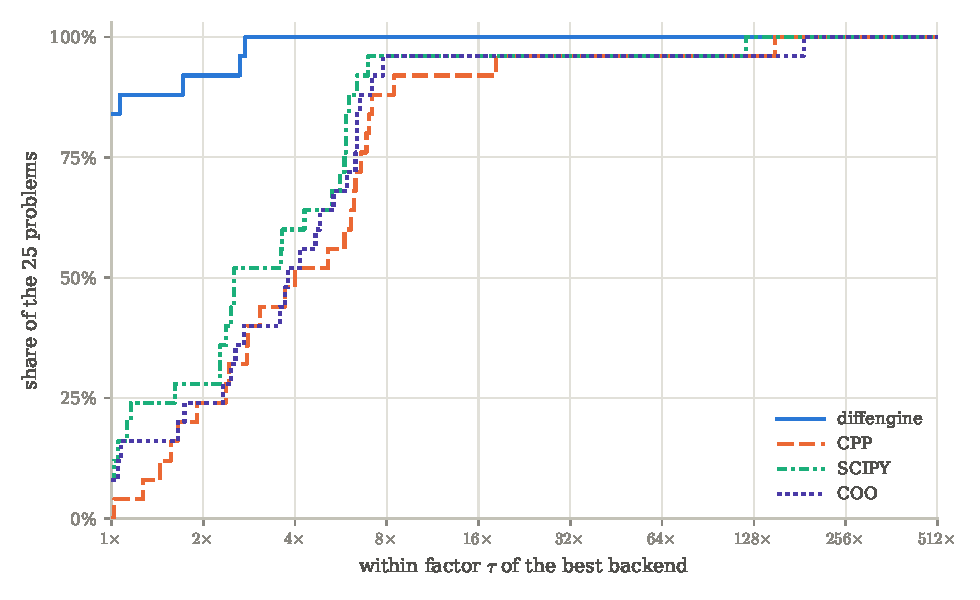
\includegraphics[width=0.72\textwidth]{performance_profile_thesis}
\end{center}

\vspace{-2.5ex}
\begin{center}\small
\de{} is within $3\times$ of the best backend on \emph{every} problem.\\[0.4ex]
{\color{black!55}\footnotesize No \cvxpy{} backend is fastest on more than two problems, and
each needs $\tau \approx 8$ to cover 92--96\% of them.}
\end{center}
\end{frame}

% ==================================================================================
\section{Parametric canonicalization}
% ==================================================================================

% --- PC0 --------------------------------------------------------------------------
%  Opens the section with the use case the whole mechanism is for, before any mechanism.
%  The problem is the one of F1 (:857) verbatim -- same objective, same x >= 0, same
%  mu = cp.Parameter(nonneg=True) -- so the only new thing on the slide is the loop around
%  it. A regularization path is the honest instance of that loop: mu is the knob the running
%  example already has, and nobody solves such a problem once.
%
%  Kept free of DPP, like the rest of the section before PC3: the slide says only that the
%  structure is identical at every iteration, which is an observation about the loop, not a
%  claim about what CVXPY does with it. PC3 is where the comparison belongs.
%
%  [fragile] is required: the frame carries an lstlisting.
%  Sources: 7-Theme2.tex (the parametric benchmarks are all sweeps of this shape),
%           5-Introduction.tex:143-144 (why solver interfaces are built around re-solves).
\begin{frame}[fragile]{The same problem, a hundred times}
\vspace{-0.5ex}
{\small A regularization path over the weight $\mu$ of the running example:}

\vspace{0.5ex}
\begin{center}
\begin{minipage}{0.86\textwidth}
\begin{lstlisting}[language=mypython, basicstyle=\ttfamily\small,
                   aboveskip=0.4em, belowskip=0.4em]
mu = cp.Parameter(nonneg=True)
prob = cp.Problem(
    cp.Minimize(cp.norm(F @ x - g) + mu * cp.norm(x)),
    [x >= 0])

for value in np.logspace(-2, 2, 100):
    mu.value = value
    prob.solve()
\end{lstlisting}
\end{minipage}
\end{center}

\vspace{1.5ex}
\begin{itemize}\small\bul
  \item same tree, same cones, same sparsity pattern at every iteration ---
        {\color{polyblue}one scalar changes}
  \item so {\color{polyblue}the structure is computed once; a re-solve is values only}
\end{itemize}
\end{frame}

% --- PC1 --------------------------------------------------------------------------
%  Deliberately free of DPP: this section presents our mechanism on its own terms, and DPP
%  is introduced once on PC3, as the thing the Results section measures against.
%  Sources: 3-Abstract.tex:26-29 (the two passes, one numeric pass per re-solve),
%           7-Theme1.tex:529-534 (the numeric pass allocates nothing),
%           5-Introduction.tex:143-144 (the idea is borrowed from NLP solver interfaces).
%  That provenance was a third bullet and is spoken: it is where the two-pass split comes
%  from, not what it does, and the two bullets that remain are what it does.
\begin{frame}{Two passes}
\vspace{-0.5ex}
{\small The sparsity patterns are fixed across a problem family: a parameter changes the
\emph{values} of the problem data, never its \emph{structure}.}

\vspace{2ex}
\begin{center}
\fitfig{%
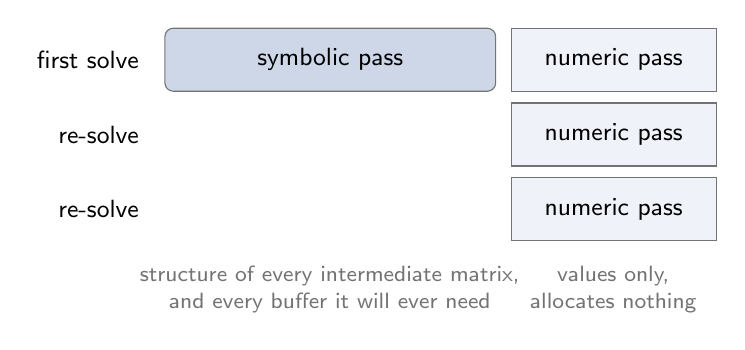
\begin{tikzpicture}[x=1cm, y=1cm]
  \node[font=\small, anchor=east] at (-0.2, 0)    {first solve};
  \node[font=\small, anchor=east] at (-0.2, -0.95) {re-solve};
  \node[font=\small, anchor=east] at (-0.2, -1.90) {re-solve};
  \node[proc, minimum width=4.2cm, anchor=west] at (0, 0)    {symbolic pass};
  \node[art,  minimum width=2.6cm, minimum height=8mm, anchor=west] at (4.4, 0)
    {numeric pass};
  \node[art,  minimum width=2.6cm, minimum height=8mm, anchor=west] at (4.4, -0.95)
    {numeric pass};
  \node[art,  minimum width=2.6cm, minimum height=8mm, anchor=west] at (4.4, -1.90)
    {numeric pass};
  \node[font=\footnotesize, text=black!55, anchor=north, align=center] at (2.1, -2.5)
    {structure of every intermediate matrix,\\and every buffer it will ever need};
  \node[font=\footnotesize, text=black!55, anchor=north, align=center] at (5.7, -2.5)
    {values only,\\allocates nothing};
\end{tikzpicture}}
\end{center}

\vspace{1.5ex}
\begin{itemize}\small\bul
  \item re-solving a parametrized problem costs {\color{polyblue}one numeric pass}
  \item {\color{polyblue}no restriction on how the parameters enter the problem}
\end{itemize}
\end{frame}

% --- PC2 --------------------------------------------------------------------------
%  The mechanism, with the worked example. fig:sum-idx-map is lifted from
%  7-Theme1.tex:619-697; its local `nz' style is renamed `sm' here, because the deck's
%  preamble already defines `nz' for the sparsity-pattern figure (I4).
%  Three-item list: 7-Theme1.tex:533-534. Closing line: 7-Theme1.tex:706-713.
\begin{frame}{What the symbolic pass stores}
\vspace{-1ex}
{\small Depending on the kernel, the stored structure is a \textbf{sparsity pattern}, a
\textbf{block layout}, or an \textbf{index map}.}

\vspace{1.5ex}
\begin{center}
\fitfig{%
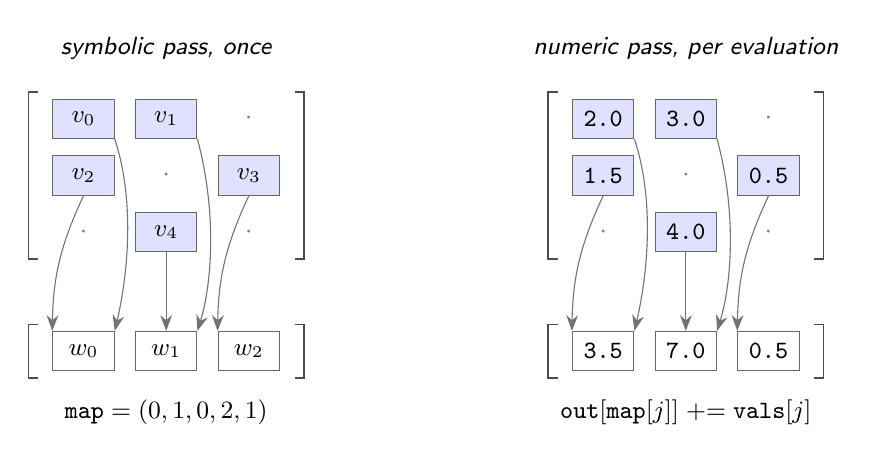
\begin{tikzpicture}[
  sm/.style={draw=black!60, fill=blue!12, minimum width=0.78cm, minimum height=0.5cm,
             font=\small\ttfamily, anchor=center},
  outc/.style={draw=black!60, minimum width=0.78cm, minimum height=0.5cm,
               font=\small\ttfamily, anchor=center},
  zero/.style={font=\normalsize, text=black!50, anchor=center},
  map/.style={-{Stealth[length=2mm]}, black!55},
  ttl/.style={font=\small\itshape, anchor=center},
  brk/.style={black!70, line width=0.5pt},
]
\def\dx{1.05}
\def\dy{0.72}
\def\oy{-2.95}
% ---------- left panel: symbolic ----------
\node[ttl] at (\dx, 0.9) {symbolic pass, once};
\node[sm] (L0) at (0, 0)          {$v_0$};
\node[sm] (L1) at (\dx, 0)        {$v_1$};
\node[zero] at (2*\dx, 0)         {$\cdot$};
\node[sm] (L2) at (0, -\dy)       {$v_2$};
\node[zero] at (\dx, -\dy)        {$\cdot$};
\node[sm] (L3) at (2*\dx, -\dy)   {$v_3$};
\node[zero] at (0, -2*\dy)        {$\cdot$};
\node[sm] (L4) at (\dx, -2*\dy)   {$v_4$};
\node[zero] at (2*\dx, -2*\dy)    {$\cdot$};
\draw[brk] (-0.58, 0.34) -- (-0.70, 0.34) -- (-0.70, -2*\dy-0.34) -- (-0.58, -2*\dy-0.34);
\draw[brk] (2*\dx+0.58, 0.34) -- (2*\dx+0.70, 0.34)
        -- (2*\dx+0.70, -2*\dy-0.34) -- (2*\dx+0.58, -2*\dy-0.34);
\node[outc] (M0) at (0, \oy)      {$w_0$};
\node[outc] (M1) at (\dx, \oy)    {$w_1$};
\node[outc] (M2) at (2*\dx, \oy)  {$w_2$};
\draw[brk] (-0.58, \oy+0.34) -- (-0.70, \oy+0.34) -- (-0.70, \oy-0.34) -- (-0.58, \oy-0.34);
\draw[brk] (2*\dx+0.58, \oy+0.34) -- (2*\dx+0.70, \oy+0.34)
        -- (2*\dx+0.70, \oy-0.34) -- (2*\dx+0.58, \oy-0.34);
\draw[map] (L0.south east) .. controls (0.66,-1.05) and (0.56,-2.0) .. (M0.north east);
\draw[map] (L1.south east) .. controls (1.70,-1.2) and (1.63,-2.1) .. (M1.north east);
\draw[map] (L2.south) to[bend right=12] (M0.north west);
\draw[map] (L3.south) to[bend right=12] (M2.north west);
\draw[map] (L4.south) -- (M1.north);
\node[font=\small, anchor=north] at (\dx, \oy-0.5)
  {$\mathtt{map} = (0, 1, 0, 2, 1)$};
% ---------- right panel: numeric ----------
\begin{scope}[xshift=6.6cm]
\node[ttl] at (\dx, 0.9) {numeric pass, per evaluation};
\node[sm] (R0) at (0, 0)          {2.0};
\node[sm] (R1) at (\dx, 0)        {3.0};
\node[zero] at (2*\dx, 0)         {$\cdot$};
\node[sm] (R2) at (0, -\dy)       {1.5};
\node[zero] at (\dx, -\dy)        {$\cdot$};
\node[sm] (R3) at (2*\dx, -\dy)   {0.5};
\node[zero] at (0, -2*\dy)        {$\cdot$};
\node[sm] (R4) at (\dx, -2*\dy)   {4.0};
\node[zero] at (2*\dx, -2*\dy)    {$\cdot$};
\draw[brk] (-0.58, 0.34) -- (-0.70, 0.34) -- (-0.70, -2*\dy-0.34) -- (-0.58, -2*\dy-0.34);
\draw[brk] (2*\dx+0.58, 0.34) -- (2*\dx+0.70, 0.34)
        -- (2*\dx+0.70, -2*\dy-0.34) -- (2*\dx+0.58, -2*\dy-0.34);
\node[outc] (S0) at (0, \oy)      {3.5};
\node[outc] (S1) at (\dx, \oy)    {7.0};
\node[outc] (S2) at (2*\dx, \oy)  {0.5};
\draw[brk] (-0.58, \oy+0.34) -- (-0.70, \oy+0.34) -- (-0.70, \oy-0.34) -- (-0.58, \oy-0.34);
\draw[brk] (2*\dx+0.58, \oy+0.34) -- (2*\dx+0.70, \oy+0.34)
        -- (2*\dx+0.70, \oy-0.34) -- (2*\dx+0.58, \oy-0.34);
\draw[map] (R0.south east) .. controls (0.66,-1.05) and (0.56,-2.0) .. (S0.north east);
\draw[map] (R1.south east) .. controls (1.70,-1.2) and (1.63,-2.1) .. (S1.north east);
\draw[map] (R2.south) to[bend right=12] (S0.north west);
\draw[map] (R3.south) to[bend right=12] (S2.north west);
\draw[map] (R4.south) -- (S1.north);
\node[font=\small, anchor=north] at (\dx, \oy-0.5)
  {$\mathtt{out[map[}j\mathtt{]]} \mathrel{+}= \mathtt{vals[}j\mathtt{]}$};
\end{scope}
\end{tikzpicture}}
\end{center}

\vspace{0.5ex}
\begin{center}\small
The \texttt{sum} atom: the symbolic pass records where each nonzero lands, the numeric pass
follows the fixed arrows.\\[0.5ex]
{\color{polyblue}\texttt{index}, \texttt{transpose} and \texttt{broadcast} build the same map,
with a copy in place of an addition.}
\end{center}
\end{frame}

% --- PC3 --------------------------------------------------------------------------
%  What we are actually compared against, stated once, just before the Results section.
%  Sources: 6-Revue_litterature.tex:383-396 (eq:param-maps, one sparse matvec per map),
%           6-Revue_litterature.tex:458-470 (the three backends and how each represents the
%           parameter axis), 6-Revue_litterature.tex:478-479 (the default-selection rule).
%  Two framing sentences came off and are spoken: "a re-solve is then one sparse
%  matrix-vector product per map", which is what the display says once it is read, and the
%  closing "the benchmarks that follow compare against all three", which is what the next
%  slide shows rather than something to announce.
\begin{frame}{The parameter maps}
\vspace{-0.5ex}
{\small Under DPP the data is affine in the parameters, so the family collapses to two
cached maps:}
\[
  \mvec{c} = \mmat{Q}\,\gvec{\tilde\theta},
  \qquad
  \vect([\mmat{A}\ \mvec{b}]) = \mmat{R}\,\gvec{\tilde\theta},
  \qquad
  \gvec{\tilde\theta} = \begin{bmatrix} \gvec{\theta} \\ 1 \end{bmatrix}
\]
\vspace{2ex}
{\small \cvxpy{}'s three backends are three representations of that same tensor:}
\begin{itemize}\small\bul
  \item \texttt{cvxcore} (C++) --- one sparse matrix per parameter slice
  \item \texttt{SCIPY} --- the slices stacked into one strided sparse matrix
  \item \texttt{COO} --- never formed: triples with a parameter index
\end{itemize}
\end{frame}

% --- R3 ---------------------------------------------------------------------------
%  tab:param-tensor, 7-Theme2.tex:165-180, verbatim (7 rows fit a slide as they are).
%  The two-regime explanation is 7-Theme2.tex:184-189.
\begin{frame}{Parametric problems}
\vspace{-1ex}
{\scriptsize\color{black!55} The seven DPP parametric problems \textbullet{} a dash is a
tensor that did not finish inside the time limit}

\vspace{1.5ex}
\begin{center}\footnotesize
\setlength{\tabcolsep}{4pt}
\begin{tabular}{@{}l rrrr rr r@{}}
\toprule
& \multicolumn{4}{c}{first canonicalization} & \multicolumn{2}{c}{re-solve} & \\
\cmidrule(lr){2-5}\cmidrule(lr){6-7}
Benchmark & \texttt{CPP} & \texttt{SCIPY} & \texttt{COO} & \de{} & tensor & \de{} & Ratio \\
\midrule
ParamSmallMatrixStuffing   &  7.78 & 29.06 &  0.40 & \textbf{0.21} & 0.005 & \textbf{0.001} & 0.29 \\
ParamConeMatrixStuffing    &  3.16 &  7.63 &  0.26 & \textbf{0.14} & 0.003 & \textbf{0.001} & 0.29 \\
SimpleFullyParametrizedLP  &   --- &   --- &  2.17 & \textbf{0.54} & 0.261 & \textbf{0.126} & 0.48 \\
ParametrizedQP             &   --- &   --- & 10.87 & \textbf{2.53} & 1.485 & \textbf{0.985} & 0.66 \\
SimpleScalarParametrizedLP &  4.68 &  4.15 &  4.48 & \textbf{1.03} & 0.304 & \textbf{0.247} & 0.81 \\
SVMWithL1Regularization    & 11.00 &  8.21 &  9.62 & \textbf{1.86} & \textbf{0.252} & 0.496 & 1.97 \\
FactorCovarianceModel      &  4.92 &  4.15 &  4.66 & \textbf{0.86} & \textbf{0.139} & 0.279 & 2.00 \\
\bottomrule
\end{tabular}
\end{center}

\vspace{1.5ex}
\begin{center}\small
Fastest first canonicalization on every problem; re-solve within about $2\times$ the tensor.
\\[0.4ex]
{\color{black!55}\footnotesize The last two: data almost all constant, and an update still
recomputes it.}
\end{center}
\end{frame}

% ==================================================================================
\section{Conclusion}
% ==================================================================================

% --- R4 ---------------------------------------------------------------------------
%  The three observations, 7-Theme2.tex:196-209, and the downsides, 7-Theme2.tex:232-236
%  and 8-Conclusion.tex:57-66. The memory numbers are 7-Theme2.tex:77-82.
\begin{frame}{Three observations}
\vspace{-0.5ex}
\begin{itemize}\small\bul
  \item {\color{polyblue}\textbf{Caching does not require the DPP ruleset.}}
        Within $\sim\!2\times$ the cached tensor, every problem.
  \item {\color{polyblue}\textbf{The tensor's upfront cost is not always justified.}}
        First canonicalization faster on all seven, re-solve on five.
  \item {\color{polyblue}\textbf{\texttt{cvxcore} can be replaced.}}
        Faster on $24$ of $25$, and on all seven parametric.
\end{itemize}

\vspace{2ex}
\onslide<2->{%
{\small\textbf{and the downsides}}
\begin{itemize}\footnotesize\bul
  \item peak memory: \texttt{SCIPY} lowest on $16$ of $25$, \de{} about $1.4\times$ it
  \item the re-solve needs the cached program in memory; a built tensor does not
  \item synthetic problems, not a standard benchmark library
\end{itemize}}
\end{frame}

% --- FW ---------------------------------------------------------------------------
%  The three directions of 8-Conclusion.tex:68-120, one line each, in the thesis's own
%  order: a package, a piece of development work, and a research question.
%  The limitations are not repeated here -- R4 just gave them, on its second beat.
%  One line each, and the payoff of each is spoken: that removing cvxcore would leave CVXPY
%  shipping no C++ binaries at all, and that the solver would get presolve and factorization
%  on the dense blocks rather than rediscovering them.
\begin{frame}{Future work}
\vspace{-0.5ex}
\begin{itemize}\small\bul
  \item a standalone \sdp{} interface: sparse Jacobians and Hessians
        {\color{polyblue}without \cvxpy{}}
  \item \de{} as the default on the \texttt{ignore\_dpp} path, \texttt{cvxcore} removed
  \item pass the {\color{polyblue}block structure} to the solver, instead of having it
        rediscovered
\end{itemize}
\end{frame}

% --- closing ----------------------------------------------------------------------
\begin{frame}
\vspace{2cm}
\begin{center}
{\Large \textbf{Thank you}} \\[2ex]
\end{center}
\vfill
\end{frame}

% =====================================================================================
%  BACKUP SLIDES (not presented). appendixnumberbeamer stops the visible frame count
%  at the Thank-you slide, so these do not inflate "slide n of N".
% =====================================================================================
\appendix
% In the appendix appendixnumberbeamer restarts the count, so a backup slide would otherwise
% read "2 / 13" in the same corner where the main deck reads "25 / 37". The word disambiguates
% the two, and "backup 7" is what someone asking for one will say out loud.
\setbeamertemplate{footline}{%
  \hfill{\scriptsize\color{black!40}%
  backup \insertframenumber\,/\,\inserttotalframenumber}\hspace{2.5ex}\vspace{1.5ex}}

% --- B-DCP ------------------------------------------------------------------------
%  Q: "what exactly are the DCP rules?"  The slide dropped from the Introduction (F1).
%  Source: 5-Introduction.tex:227-250 (compliance, composition rules) and the atom table
%  at :178-197, cut down to five rows.
%  Overlaps F3e, which is in the main deck and shows six rows of the same table: that frame
%  answers "what is an atom?" and states only the two clauses the running example uses. This
%  one answers "what exactly are the rules?" -- all three clauses, the DCP-compliance
%  conditions, and the sufficient-not-necessary caveat. Keep both; the overlap is the table,
%  and it is four rows of it.
\begin{frame}{Backup: the DCP rules}
\vspace{-0.5ex}
{\small Every atom declares its curvature, its monotonicity in each argument, and the sign of
its output:}
\vspace{0.5ex}
\begin{center}\footnotesize
\begin{tabular}{l l l l l}
\toprule
Atom & Definition & Curvature & Monotonicity & Sign \\
\midrule
\texttt{sum}    & $\textstyle\sum_i x_i$ & affine  & non-decreasing & any \\
\texttt{abs}    & $|x|$                  & convex  & unknown        & nonnegative \\
\texttt{square} & $x^2$                  & convex  & unknown        & nonnegative \\
\texttt{sqrt}   & $\sqrt{x}$             & concave & non-decreasing & nonnegative \\
\texttt{norm}   & $\|\mvec{x}\|_2$       & convex  & unknown        & nonnegative \\
\bottomrule
\end{tabular}
\end{center}

\vspace{1ex}
{\small The composition $\phi(u_1(\mvec{x}), \dots, u_k(\mvec{x}))$ is
{\color{polyblue}convex} when $\phi$ is convex and, for {\color{polyblue}each} argument $i$,
one of the following holds:}
\vspace{-0.5ex}
\begin{itemize}\small
  \item $\phi$ is non-decreasing in $i$ and $u_i$ is convex;
  \item $\phi$ is non-increasing in $i$ and $u_i$ is concave; or
  \item $u_i$ is affine.
\end{itemize}
\vspace{0.5ex}
{\small Swap convex and concave for the concave rule. A problem is DCP-compliant when the
objective and every constraint come out compatible: convex objective,
convex $\le$ concave, affine equalities.}

\vspace{1ex}
\begin{center}\small
The rules are sufficient for convexity, not necessary: a genuinely convex problem written in an
unrecognized form is rejected.
\end{center}
\end{frame}

% --- B-NONDCP ---------------------------------------------------------------------
%  Q: "give me a problem the rules reject."  The textbook one. The composition analysis is
%  the rule set of the previous slide applied to sqrt(x^2+1); the rewrite is the SOC
%  reformulation of the norm atom, 5-Introduction.tex:283-288.
\begin{frame}[fragile]{Backup: sufficient, not necessary}
\vspace{-0.5ex}
{\small The same function, written two ways. Only one of them compiles.}
\vspace{0.5ex}
\[
  \sqrt{x^2 + 1} \;=\; \bigl\| (x,\ 1) \bigr\|_2
\]
\vspace{-2ex}
\begin{columns}[T,onlytextwidth]
\begin{column}{0.48\textwidth}
\begin{lstlisting}[language=mypython, basicstyle=\ttfamily\scriptsize,
                   aboveskip=0.4em, belowskip=0.4em]
cp.sqrt(cp.square(x) + 1)
\end{lstlisting}
\vspace{0.5ex}
{\footnotesize\color{polyblue}\textbf{rejected}}
\begin{itemize}\footnotesize
  \item \texttt{sqrt} is concave and non-decreasing
  \item its argument $x^2 + 1$ is convex, not affine
  \item no rule covers concave $\circ$ convex, so the curvature is unknown
\end{itemize}
\end{column}
\begin{column}{0.48\textwidth}
\begin{lstlisting}[language=mypython, basicstyle=\ttfamily\scriptsize,
                   aboveskip=0.4em, belowskip=0.4em]
cp.norm(cp.hstack([x, 1]))
\end{lstlisting}
\vspace{0.5ex}
{\footnotesize\color{polyblue}\textbf{accepted}}
\begin{itemize}\footnotesize
  \item \texttt{norm} is convex
  \item its argument $(x, 1)$ is affine
  \item convex $\circ$ affine is convex, and the epigraph is
        $(t,\ x,\ 1) \in \cone{K}_{\mathrm{soc},3}$
\end{itemize}
\end{column}
\end{columns}

\vspace{1.5ex}
\begin{center}\small
The rules are a test on the expression, not on the function. Rewriting is the user's job; the
atom library is what makes it possible.
\end{center}
\end{frame}

% --- B-WHYCVXPY -------------------------------------------------------------------
%  Q: "why CVXPY and not one of the other four?"  A slide of the Introduction until the
%  2026-09-20 pass, sitting between F2 and F0 and doing the narrowing on its own. F2 now
%  makes that narrowing on a bullet -- CVXPY alone, in polyblue, named aloud as the one this
%  thesis targets -- so what is left here is the evidence for it, which is worth having to
%  hand and not worth twenty seconds of a 30-minute talk.
%
%  The consequence -- every one of these installs pays the backend cost -- is spoken on F2,
%  not written: I1b lights that arrow and I5 states the goal after it.
%
%  The numbers are rounded down from what the sources gave on 2026-09-16 (6.46 M
%  downloads in August 2026 without mirrors, 6335 stars, 1215 forks), so they stay true
%  if anyone re-checks them on the day. The trailing-30-day figure was higher, 7.18 M;
%  the calendar month is the safer one to say out loud. The growth -- 3.7 M in April to
%  6.5 M in August 2026 -- is worth saying, not worth putting on the slide: pypistats
%  retains only 180 days, so the series starts in March 2026 and five months is not a
%  trend to stand on.
%
%  Plain bullets in F2's shape, not a figure: two reasons and two numbers do not need a
%  picture, and the two slides either side of this one are both full-width TikZ.
%
%  Bullet 1 is the reach, bullet 2 the maturity and the volume, bullet 3 the standing.
%  The stars and forks (6.3 k / 1.2 k) were a fourth bullet and came off: they measure the
%  same reach the download count already measures, and five numbers on one slide is four
%  more than anyone retains. Say them if the floor asks how active the project is.
%  Open source matters here beyond goodwill: it is why the backend can be replaced at all,
%  which is what R4 claims in the Conclusion. The licence is Apache 2.0 today -- the 2016
%  paper says GPL, so do not quote the paper on the licence.
%  Python at number one is TIOBE's ranking, September 2026 -- hence the index in the source
%  line; GitHub's Octoverse and the Stack Overflow survey agree, so the claim does not rest
%  on one source.
%
%  "Over ten years" is understated on purpose, the way the other figures are: the repo was
%  created in July 2013 and the first PyPI release (0.1) is May 2014, so thirteen and twelve
%  years respectively, across 148 releases with the latest in June 2026. Say "over ten" and
%  nobody can take issue with it.
%
%  The 4.5 k is Google Scholar's count for Diamond and Boyd (2016), which is the figure
%  usually quoted for that paper. Do not "correct" it downwards against OpenAlex: OpenAlex
%  splits the JMLR record from the arXiv preprint and gives 683 + 477, an undercount of a
%  paper that is cited far more widely than either record sees.
%
%  Sources: 3-Abstract.tex:14 ("widely used modelling language"), 5-Introduction.tex:22
%           ("gained popularity") -- the two places the thesis asserts this with no number.
\begin{frame}{Backup: why \cvxpy{}}
\vspace{-0.5ex}
\begin{itemize}\small\bul
  \item open source, embedded in Python, the most widely used programming language
  \item in development for over ten years, over 6 million downloads a month from PyPI
  \item 4.5 k citations of the 2016 \cvxpy{} paper
\end{itemize}
\vfill
{\scriptsize\color{black!55} TIOBE index, \texttt{pypistats.org},
\texttt{github.com/cvxpy/cvxpy} and Google Scholar, September 2026.}
\end{frame}
% --- B-DPP ------------------------------------------------------------------------
%  Q: "what is DPP, and why does the tensor backend need it?"
%  Source: 6-Revue_litterature.tex:376-397 (the grammar, the maps, the third tensor
%  dimension) and :423-431 (the ignore_dpp path).
\begin{frame}{Backup: disciplined parametrized programming}
\vspace{-0.5ex}
{\small DPP is a second grammar, on top of DCP, restricting how parameters may enter an
expression: every parameter is treated as affine, and products of two parametrized expressions
are forbidden.}

\vspace{1ex}
{\small The payoff is that the problem data becomes {\color{polyblue}affine in the
parameters}:}
\[
  \mvec{c} = \mmat{Q}\,\gvec{\tilde\theta},
  \qquad
  \vect([\mmat{A}\ \mvec{b}]) = \mmat{R}\,\gvec{\tilde\theta},
  \qquad
  \gvec{\tilde\theta} = \begin{bmatrix} \gvec{\theta} \\ 1 \end{bmatrix}
\]

\vspace{0.5ex}
\begin{itemize}\small\bul
  \item \cvxpy{} builds $\mmat{Q}$ and $\mmat{R}$ by adding a third dimension to every
        coefficient matrix of the pass, indexed by the parameter entries
  \item after a parameter change, a re-solve costs one sparse matrix-vector product per map:
        no tree is traversed again
  \item a problem outside the grammar, or one passing \texttt{ignore\_dpp}, takes the
        \texttt{EvalParams} path instead: each parameter leaf is replaced by its current value
        and the whole canonicalization repeats
\end{itemize}

\vspace{1ex}
\begin{center}\small
This is the baseline the parametric results are measured against.
\end{center}
\end{frame}

% --- B-OTHERLANG ------------------------------------------------------------------
%  Q: "how is this different from JuMP / AMPL / CasADi?"
%  Source: 6-Revue_litterature.tex:1055-1074 (the two families and the parameter handling).
\begin{frame}{Backup: two ways to get the coefficients}
\vspace{-0.5ex}
{\small Every modelling language reviewed produces the same output, the solver problem data. They
split into two families by what they ask of the user.}

\vspace{1.5ex}
{\small\color{polyblue}\textbf{Differentiate an expression graph}}
\begin{itemize}\small
  \item \texttt{CasADi}: built for nonlinear optimization; its conic interface \texttt{qpsol}
        differentiates the graph through matrix-vector products, so the sparsity pattern must be
        {\color{polyblue}detected at runtime} and compressed by colouring
  \item \cvxpy{}: composes the linear operators of the conic-form trees in one bottom-up pass,
        which is equivalent to differentiating them; expressions stay vectorized, so no detection
        step is needed
  \item {\color{polyblue}\sde{}}: differentiates them outright, one Jacobian per node with
        respect to \emph{all} the variables, so the chain rule is a single matrix product ---
        not a dictionary of blocks keyed by variable
\end{itemize}

\vspace{1ex}
{\small\color{polyblue}\textbf{Read the coefficients the user declares}}
\begin{itemize}\small
  \item \texttt{AMPL}, \texttt{JuMP}: the user writes each objective and constraint as a sum of
        terms, and every linear and quadratic coefficient is stored as it is typed
  \item neither has an atom library or a canonicalization step, so a norm is left to the solver
        (\texttt{AMPL}) or written in conic form by hand (\texttt{JuMP}); both scalarize
\end{itemize}
\end{frame}

% --- B-GAP ------------------------------------------------------------------------
%  Q: "so what is actually new?"  tab:systems-summary, 6-Revue_litterature.tex:1084-1131,
%  with the acronyms spelled out (the deck does not load the acronym package).
\begin{frame}{Backup: the research gap}
\vspace{-1ex}
\begin{center}
\adjustbox{max size={0.98\textwidth}{0.62\textheight}}{%
\footnotesize
\setlength{\tabcolsep}{5pt}
\begin{tabular}{@{}l >{\raggedright\arraybackslash}p{1.9cm} >{\raggedright\arraybackslash}p{3.0cm}
  >{\raggedright\arraybackslash}p{3.1cm} >{\raggedright\arraybackslash}p{2.9cm}@{}}
\toprule
\textbf{System} & \textbf{Expression storage} & \textbf{Coefficients obtained by}
  & \textbf{Reused across the family} & \textbf{Repeated at every solve} \\
\midrule
\texttt{AMPL}
  & scalar
  & instance generation
  & nothing, values folded into the instance
  & \texttt{.nl} write and read \\
\arrayrulecolor{black!30}\specialrule{0.3pt}{1.5pt}{1.5pt}\arrayrulecolor{black}
\texttt{JuMP}
  & scalar
  & term lists stored by macros
  & term lists, modified in place
  & \texttt{copy\_to} into the solver \\
\arrayrulecolor{black!30}\specialrule{0.3pt}{1.5pt}{1.5pt}\arrayrulecolor{black}
\texttt{CasADi}
  & scalar or matrix
  & differentiation of an expression graph
  & pattern, colouring, derivative function
  & one sweep per colour \\
\arrayrulecolor{black!30}\specialrule{0.3pt}{1.5pt}{1.5pt}\arrayrulecolor{black}
\cvxpy{} backends
  & vectorized
  & composition of linear operators
  & parameter-to-data tensor, DPP problems only
  & one tensor-vector product, or the whole pass \\
\arrayrulecolor{black!30}\specialrule{0.3pt}{1.5pt}{1.5pt}\arrayrulecolor{black}
{\color{polyblue}\sde{}}
  & {\color{polyblue}vectorized}
  & {\color{polyblue}structured direct differentiation}
  & {\color{polyblue}problem structure, by the symbolic pass}
  & {\color{polyblue}numeric pass} \\
\bottomrule
\end{tabular}}
\end{center}

\vspace{0.5ex}
\begin{center}\small
None of the four combines the two-phase split with direct computation of the problem data.\\[0.4ex]
{\color{black!55}\footnotesize Two phases like \texttt{CasADi}, but the whole coefficient matrix
at once instead of matrix-vector products, and dense storage where the structure is dense.}
\end{center}
\end{frame}

% --- SUM --------------------------------------------------------------------------
%  Q: "how much code is this, and how many derivative rules did you have to write?"
%  Was the opening frame of the Conclusion, where it was the densest slide in the deck and
%  the only method content after the results. Moved here: the whole library is ten kernels,
%  and the contribution is that each one dispatches to the representation in front of it
%  rather than flattening everything to one format -- a good answer to a question, and too
%  much to read aloud in a 30-minute slot.
%  Sources: tab:kernel-operations at 7-Theme1.tex:386-411 (the ten kernels, verbatim minus
%           the "Called by" column, which the prose carries instead),
%           7-Theme1.tex:413-437 (unary vs binary dispatch, double dispatch on the transposed
%           products, addition always in CSR),
%           7-Theme1.tex:493-503 (the four kernel families, and "once a dense block appears,
%           the dense representations take over").
\begin{frame}{Backup: ten kernels is the whole library}
\vspace{-1ex}
\begin{columns}[T,onlytextwidth]
\begin{column}{0.47\textwidth}
\vspace{1ex}
\centering
{\footnotesize
\begin{tabular}{@{}ll@{}}
\toprule
Kernel & Computes \\
\midrule
\texttt{transpose}          & $\mmat{A}^\top$ \\
\texttt{index}              & $\mmat{A}[\mvec{r}, :]$ \\
\texttt{sum\_row\_partition}& sums of groups of rows \\
\texttt{promote}            & copies of a single row \\
\texttt{broadcast}          & copies of a row or a column \\
\texttt{diag\_vec}          & rows moved to the diagonal \\
\texttt{DA}                 & $\diag(\mvec{d})\,\mmat{A}$ \\
\midrule
\texttt{sum\_matrices}      & $\mmat{A} + \mmat{B}$ \\
\texttt{BA}                 & $\mmat{B}\mmat{A}$ \\
\texttt{BTA}, \texttt{BTDA} & $\mmat{B}^\top\mmat{A}$,\ \ $\mmat{B}^\top\mmat{D}\mmat{A}$ \\
\bottomrule
\end{tabular}}

\vspace{1ex}
{\scriptsize\color{black!55} seven unary, three binary}
\end{column}
\begin{column}{0.50\textwidth}
\begin{itemize}\small\bul
  \item every atom of a canonicalized DCP problem reaches its derivative through one of these
        --- there is no per-atom derivative code to write
  \item each kernel is written once {\color{polyblue}per representation}, and the call selects
        the implementation: the unary ones on their operand, the transposed products on
        {\color{polyblue}both} operands at once
  \item so dense and sparse {\color{polyblue}mix freely}: a sparse-dense pair is a kernel that
        converts neither operand, and a product with a dense operand gives back a dense one
  \item once a dense block appears, the dense path takes over and the structure is never
        flattened into $(\text{row}, \text{column}, \text{value})$ triples
\end{itemize}
\end{column}
\end{columns}

\vspace{1ex}
\begin{center}\small\color{polyblue}
Being free to pick the representation per operation is what the timings measure.
\end{center}
\end{frame}

% --- SUM1b ------------------------------------------------------------------------
%  Q: "what happens when the variable is a matrix?"  The third representation, which the
%  main line deliberately never names: SC2 ends on the permuted dense triple and stops.
%  Sits immediately before the dispatch table, whose sPD row and column are meaningless
%  without it.
%
%  The figure is the thesis's own, fig:stacked-pd at 7-Theme1.tex:349-374, kept at its size
%  (4 x 10, two 2 x 2 blocks) so it reads against SC2's picture: same ten columns, same
%  b_{ij}, one block there and two here. Tints are the thesis's local pdRowB/pdRowC, one per
%  block rather than one per row -- the correspondence being shown here is block to block.
%
%  NOT inside \fitfig: nicematrix's \CodeBefore panels are placed with absolute coordinates
%  and a scalebox displaces them (the same trap as SC2).
%  Sources: 7-Theme1.tex:335-360 (why neither a bigger block nor the sparse form will do,
%           and the single shared value buffer).
\colorlet{pdRowB}{green!16!white}
\colorlet{pdRowC}{orange!22!white}
\begin{frame}{Backup: when the variable is a matrix}
\vspace{-0.5ex}
{\footnotesize Multiplying a matrix variable $\mmat{V} \in \reals^{2\times2}$ by dense
$\mmat{B}$ acts on each column separately: one dense block per column of $\mmat{V}$, at
disjoint rows and different columns.}

\vspace{0.5ex}
\begin{center}
{\small
$\mmat{M} =
\begin{pNiceMatrix}[margin]
\CodeBefore
  \rectanglecolor{pdRowB}{1-5}{2-6}
  \rectanglecolor{pdRowC}{3-7}{4-8}
\Body
\cdot & \cdot & \cdot & \cdot & b_{00} & b_{01} & \cdot  & \cdot  & \cdot & \cdot \\
\cdot & \cdot & \cdot & \cdot & b_{10} & b_{11} & \cdot  & \cdot  & \cdot & \cdot \\
\cdot & \cdot & \cdot & \cdot & \cdot  & \cdot  & b_{00} & b_{01} & \cdot & \cdot \\
\cdot & \cdot & \cdot & \cdot & \cdot  & \cdot  & b_{10} & b_{11} & \cdot & \cdot
\end{pNiceMatrix}$}
\end{center}

\vspace{0.5ex}
\begin{center}\small
$\mmat{X}_1 = \mmat{X}_2 = \mmat{B}, \qquad
 \mvec{r}_1 = (0,1),\ \mvec{c}_1 = (4,5), \qquad
 \mvec{r}_2 = (2,3),\ \mvec{c}_2 = (6,7)$
\end{center}

\vspace{1.5ex}
\begin{itemize}\footnotesize\bul
  \item no single triple describes this: merging the blocks would store the zeros between
        them, and the generic sparse form would lose the dense structure
  \item a {\color{polyblue}stacked} permuted dense matrix is the vertical union of blocks at
        pairwise disjoint rows --- every operation treats them one at a time, and the global
        matrix is never formed
  \item the stack owns one value buffer and each block points into it, so
        $\mmat{B}$ is stored once however many columns $\mmat{V}$ has
\end{itemize}
\end{frame}

% --- SUM2 -------------------------------------------------------------------------
%  Q: "what actually runs when a dense block meets a sparse matrix?"  The 3 x 3 dispatch
%  table, cut from SC3 (see the note there). It is kept verbatim from the version that was
%  on the main line, except that sPD is spelled out in a line under the table: on the main
%  line SC2 had described that representation without naming it, and a backup frame has to
%  stand on its own.
%  Source: 7-Theme1.tex:440-492 (fig:kernel-dispatch, redrawn smaller for the slide).
\begin{frame}{Backup: which kernel runs on which pair}
\vspace{-0.5ex}
{\footnotesize PD is a dense block at permuted positions $(\mmat{X}, \mvec{r}, \mvec{c})$;
sPD is the stack of such blocks of the previous slide. Written out, the product of two
permuted dense matrices is}
\vspace{-1.5ex}
\[
  {\small\mmat{B}^\top \mmat{A} = \mmat{S}_{c_B}^\top \mmat{X}_B^\top
  \underbrace{\left(\mmat{S}_{r_B} \mmat{S}_{r_A}^\top\right)}_{\mathclap{\text{index-set
  intersection}}}
  \mmat{X}_A \mmat{S}_{c_A}.}
\]

\vspace{1ex}
\begin{center}
\fitfig{%
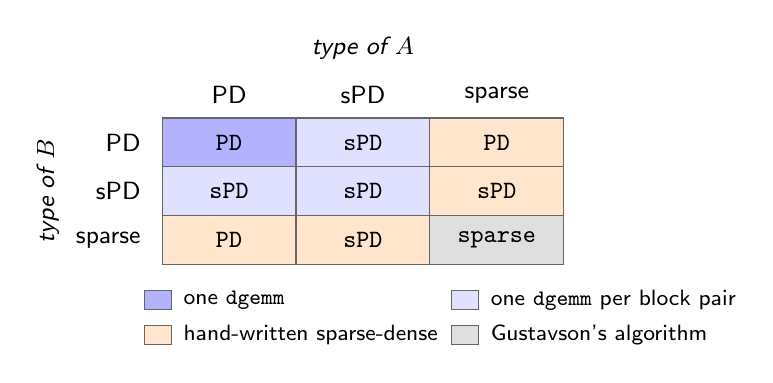
\begin{tikzpicture}[
  cell/.style={draw=black!60, minimum width=1.7cm, minimum height=0.62cm,
               font=\small\ttfamily, anchor=center},
  blas/.style={cell, fill=blue!30},
  bblas/.style={cell, fill=blue!12},
  mixed/.style={cell, fill=orange!20},
  hand/.style={cell, fill=gray!25},
  hdr/.style={font=\small, anchor=center},
]
\def\dx{1.7}
\def\dy{0.62}
\node[font=\small\itshape] at (\dx, 1.2) {type of $\mmat{A}$};
\node[hdr] at (0, 0.6) {PD};  \node[hdr] at (\dx, 0.6) {sPD};
\node[hdr] at (2*\dx, 0.6) {sparse};
\node[font=\small\itshape, rotate=90] at (-2.3, -\dy) {type of $\mmat{B}$};
\node[hdr, anchor=east] at (-1.0, 0)      {PD};
\node[hdr, anchor=east] at (-1.0, -\dy)   {sPD};
\node[hdr, anchor=east] at (-1.0, -2*\dy) {sparse};
\node[blas]  at (0, 0)          {PD};
\node[bblas] at (\dx, 0)        {sPD};
\node[mixed] at (2*\dx, 0)      {PD};
\node[bblas] at (0, -\dy)       {sPD};
\node[bblas] at (\dx, -\dy)     {sPD};
\node[mixed] at (2*\dx, -\dy)   {sPD};
\node[mixed] at (0, -2*\dy)     {PD};
\node[mixed] at (\dx, -2*\dy)   {sPD};
\node[hand]  at (2*\dx, -2*\dy) {sparse};
% legend: two columns, the right one clear of the longest left-hand label
\node[blas,  minimum width=0.34cm, minimum height=0.24cm] at (-0.9, -2.0) {};
\node[font=\footnotesize, anchor=west] at (-0.7, -2.0) {one \texttt{dgemm}};
\node[bblas, minimum width=0.34cm, minimum height=0.24cm] at (3.0, -2.0) {};
\node[font=\footnotesize, anchor=west] at (3.2, -2.0) {one \texttt{dgemm} per block pair};
\node[mixed, minimum width=0.34cm, minimum height=0.24cm] at (-0.9, -2.45) {};
\node[font=\footnotesize, anchor=west] at (-0.7, -2.45) {hand-written sparse-dense};
\node[hand,  minimum width=0.34cm, minimum height=0.24cm] at (3.0, -2.45) {};
\node[font=\footnotesize, anchor=west] at (3.2, -2.45) {Gustavson's algorithm};
\end{tikzpicture}}
\end{center}

\vspace{-1ex}
\begin{center}\small\color{polyblue}
Eight of the nine kernels come out dense; cost depends on block size, not on $m$ and $n$.
\end{center}
\end{frame}

% --- B1 ---------------------------------------------------------------------------
%  Q: "permuted dense cannot be closed under addition, surely?"  Source: 7-Theme1.tex:325-331.
\begin{frame}{Backup: addition is where the dense path stops}
\vspace{-0.5ex}
\begin{itemize}\small\bul
  \item the Jacobian of $\mmat{F}\mvec{x} + \mvec{y}$ holds the block of $\mmat{F}$ at the
        columns of $\mvec{x}$ \emph{and} an identity at the columns of $\mvec{y}$
  \item no single triple $(\mmat{X}, \mvec{r}, \mvec{c})$ covers both, so the sum is performed
        on CSR views of the two operands instead
  \item the views are built during the symbolic pass and their value arrays point at the dense
        blocks, so {\color{polyblue}no values are copied}
  \item the result is a generic sparse matrix, and so is everything computed from it
\end{itemize}

\vspace{2ex}
\begin{center}\small
The dense representations are sticky in the other direction: a product with a permuted dense or
stacked operand gives back a matrix of the same kind.
\end{center}
\end{frame}

% --- B-LOSS -----------------------------------------------------------------------
%  Q: "which of the 25 do you lose, and why?"  Was a presented frame between R1 and R2, which
%  spent a full slide of a 30-minute slot on a loss. R1's closing footnote already names both
%  losses and gives the reason, so the frame is the answer to a question rather than something
%  to walk through; it is only needed if the question is actually asked.
%
%  SDPSegfault1132 rather than ConvexPlasticity, though ConvexPlasticity has the worse ratio
%  (2.48 vs 1.39): its absolute times are 0.35 s against 0.85 s, which invites "half a second"
%  as the reply and loses the point, and its source needs the plasticity physics explained
%  before the code means anything. SDPSegfault1132 is ten lines, is a recognizable SDP, and
%  its constants are visibly dense on the slide -- V is 100 x 99, D and W are 100 x 100, and
%  V @ G @ V.T sandwiches a PSD variable between two of them three times over.
%
%  Code trimmed from benchmark/sdp_segfault_1132_benchmark.py in cvxpy/benchmarks: the
%  construction of D, V and points is replaced by comments giving their shapes, since the
%  shapes are the whole content and the arithmetic that builds them is not. The name is the
%  suite's own (it was filed as a segfault report, cvxpy issue 1132) -- kept as-is so it
%  matches the table on the previous slide. p='fro' uses single quotes: the deck is OT1 and
%  \textquotedbl is unavailable there, so a double quote in a listing is a compile error.
%
%  Sources: 7-Theme2.tex:56-59 (the two losses and the reason), tab:oneshot-compile
%           (7-Theme2.tex:119) for the timings quoted.
\begin{frame}[fragile]{Backup: a problem we do not win}
\vspace{-1ex}
{\scriptsize\color{black!55} \texttt{SDPSegfault1132}, one of the two problems of the suite
where \de{} is behind}

\vspace{0.5ex}
\begin{center}
\begin{minipage}{0.82\textwidth}
\begin{lstlisting}[language=mypython, basicstyle=\ttfamily\small,
                   aboveskip=0.4em, belowskip=0.4em]
n = 100
V = ...                      # dense, (n, n-1)
D = ...                      # dense, (n, n)
W = np.ones((n, n))          # dense, (n, n)

G = cp.Variable((n-1, n-1), PSD=True)
A = cp.kron(e,   cp.reshape(cp.diag(V @ G @ V.T), (1, n)))
B = cp.kron(e.T, cp.reshape(cp.diag(V @ G @ V.T), (n, 1)))
C = cp.norm(cp.multiply(W, A + B - 2 * V @ G @ V.T - D), p='fro')

prob = cp.Problem(cp.Maximize(cp.trace(G) - C))
\end{lstlisting}
\end{minipage}
\end{center}

\vspace{0.5ex}
\begin{itemize}\small\bul
  \item every constant is dense, and \texttt{V @ G @ V.T} sandwiches the variable between
        two of them
  \item \de{} takes $13.21$ s against \texttt{SCIPY}'s $9.51$ s: processing the dense
        constant data dominates
\end{itemize}
\end{frame}

% --- B3 ---------------------------------------------------------------------------
%  Q: "what does your caching cost you?"  Source: 8-Conclusion.tex:57-66. The one place the
%  tensor is genuinely better -- say it first.
\begin{frame}{Backup: what the two-phase split costs}
\vspace{-0.5ex}
\begin{itemize}\small\bul
  \item the numeric pass re-evaluates the expression trees at every parameter change, so the
        \texttt{problem} object must stay in memory for the lifetime of the problem family
  \item the parameter-to-data tensor has no such constraint: once it is built, a re-solve needs
        only its product with the current parameter values, and the formulation can be set aside
  \item a parameter update also forces the numeric pass to recompute the entire constant part of
        the problem data, which is why the two problems with almost-constant data and a few
        scalar parameters re-solve faster through the tensor
\end{itemize}

\vspace{2ex}
\begin{center}\small\color{polyblue}
This is the one place the tensor is genuinely the better object.
\end{center}
\end{frame}

% --- B3 ---------------------------------------------------------------------------
%  The definition dropped from the Results profile slide. Source: 7-Theme2.tex:61-75
%  (eq:perf-profile and the reading of the two ends of the curve).
\begin{frame}{Backup: how to read a performance profile}
\vspace{-0.5ex}
{\small A performance profile compares the backends over the whole suite at once, rather than
one problem at a time.}

\vspace{2ex}
\[
  f_s(\tau) = \frac{1}{n}\,\bigl|\{\, p : t_{p,s} \le \tau \textstyle\min_b t_{p,b}
  \,\}\bigr|
\]

\vspace{1ex}
\begin{itemize}\small\bul
  \item $t_{p,s}$ is the time of backend $s$ on problem $p$, and $\min_b t_{p,b}$ is the time
        of the fastest backend on that same problem
  \item $f_s(\tau)$ is the fraction of the $n$ problems on which backend $s$ lands within a
        factor $\tau$ of that best time
  \item {\color{polyblue}at $\tau = 1$}: the fraction of problems on which the backend is
        outright fastest
  \item {\color{polyblue}where the curve reaches $1$}: the factor the backend needs in order to
        cover every problem in the suite
\end{itemize}

\vspace{1.5ex}
{\scriptsize\color{black!55} Dolan and Mor\'e (2002).}
\end{frame}

% --- B4 ---------------------------------------------------------------------------
%  Panel (b) of fig:profiles. Source: 7-Theme2.tex:77-82.
%  NOTE: the standalone memory_profile_thesis.pdf labels its x axis "within factor tau of the
%  best backend", where panel (b) of the combined figure says "lowest-memory backend". That
%  discrepancy is in the source figures, not introduced here.
\begin{frame}{Backup: peak memory}
\vspace{-0.5ex}
{\small The same profile with $t_{p,s}$ replaced by the growth of the process's peak resident
memory during canonicalization:}
\vspace{-0.5ex}
\begin{center}
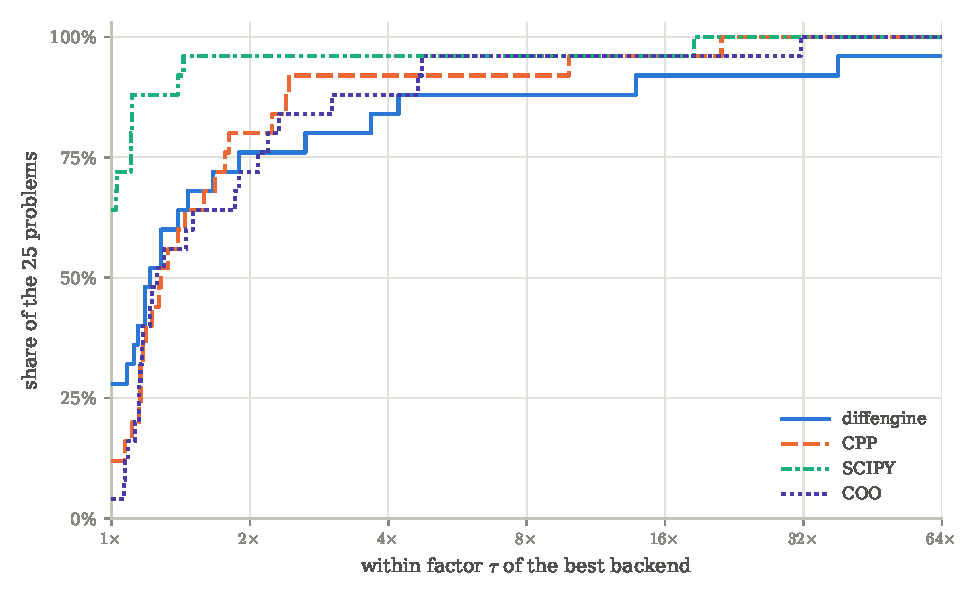
\includegraphics[width=0.66\textwidth]{memory_profile_thesis}
\end{center}

\vspace{-1ex}
\begin{center}\small
\texttt{SCIPY} has the lowest peak memory on $16$ of the $25$ problems.\\[0.4ex]
{\color{black!55}\footnotesize \de{} matches \texttt{CPP} and \texttt{COO} in geometric mean,
and uses about $1.4\times$ the memory of \texttt{SCIPY}.}
\end{center}
\end{frame}

\end{document}
